\documentclass[a4paper,fleqn]{cas-dc}

\usepackage[authoryear,longnamesfirst]{natbib}
\usepackage{amssymb}
\usepackage{graphicx}
\usepackage{url}
\usepackage{placeins}
\usepackage{pdfpages}
\usepackage{algorithm}
\usepackage[noend]{algpseudocode}
% A figure set in the text, not floated: cas-dc's figure environment ignores [H]. Uses cas-dc's own figure caption style.
\makeatletter
\ExplSyntaxOn
\newenvironment{inlinefigure}
  { \par\medskip\noindent\begin{minipage}{\columnwidth}
    \def\@captype{figure}
    \__reset_fig:
    \dim_set:Nn \l_fig_width_dim { \linewidth }
    \cs_set_eq:NN \@makecaption \__make_fig_caption:nn
    \centering\sffamily\small }
  { \end{minipage}\par\medskip }
\ExplSyntaxOff
\makeatother
\usepackage{booktabs}
% a float gets a page of its own only when it fills most of it; otherwise it goes at the top of a text page
\renewcommand{\topfraction}{0.9}
\renewcommand{\dbltopfraction}{0.9}
\renewcommand{\textfraction}{0.1}
\renewcommand{\floatpagefraction}{0.8}
\renewcommand{\dblfloatpagefraction}{0.8}
\usepackage{xcolor}
\newcommand{\confirm}[1]{\textcolor{red}{#1 [authors to confirm]}}
\setlength{\emergencystretch}{2em}
\RenewDocumentCommand{\printorcid}{}{} % cas-dc prints an empty "ORCID(s):" footnote when no ORCID is given % lets long \texttt{} words break without running into the margin

\begin{document}
\let\WriteBookmarks\relax
\def\floatpagepagefraction{1}
\def\textpagefraction{.001}

% CEP handout: the grading rubric (names filled in by make_rubric.py) and a title page go in front of the report.
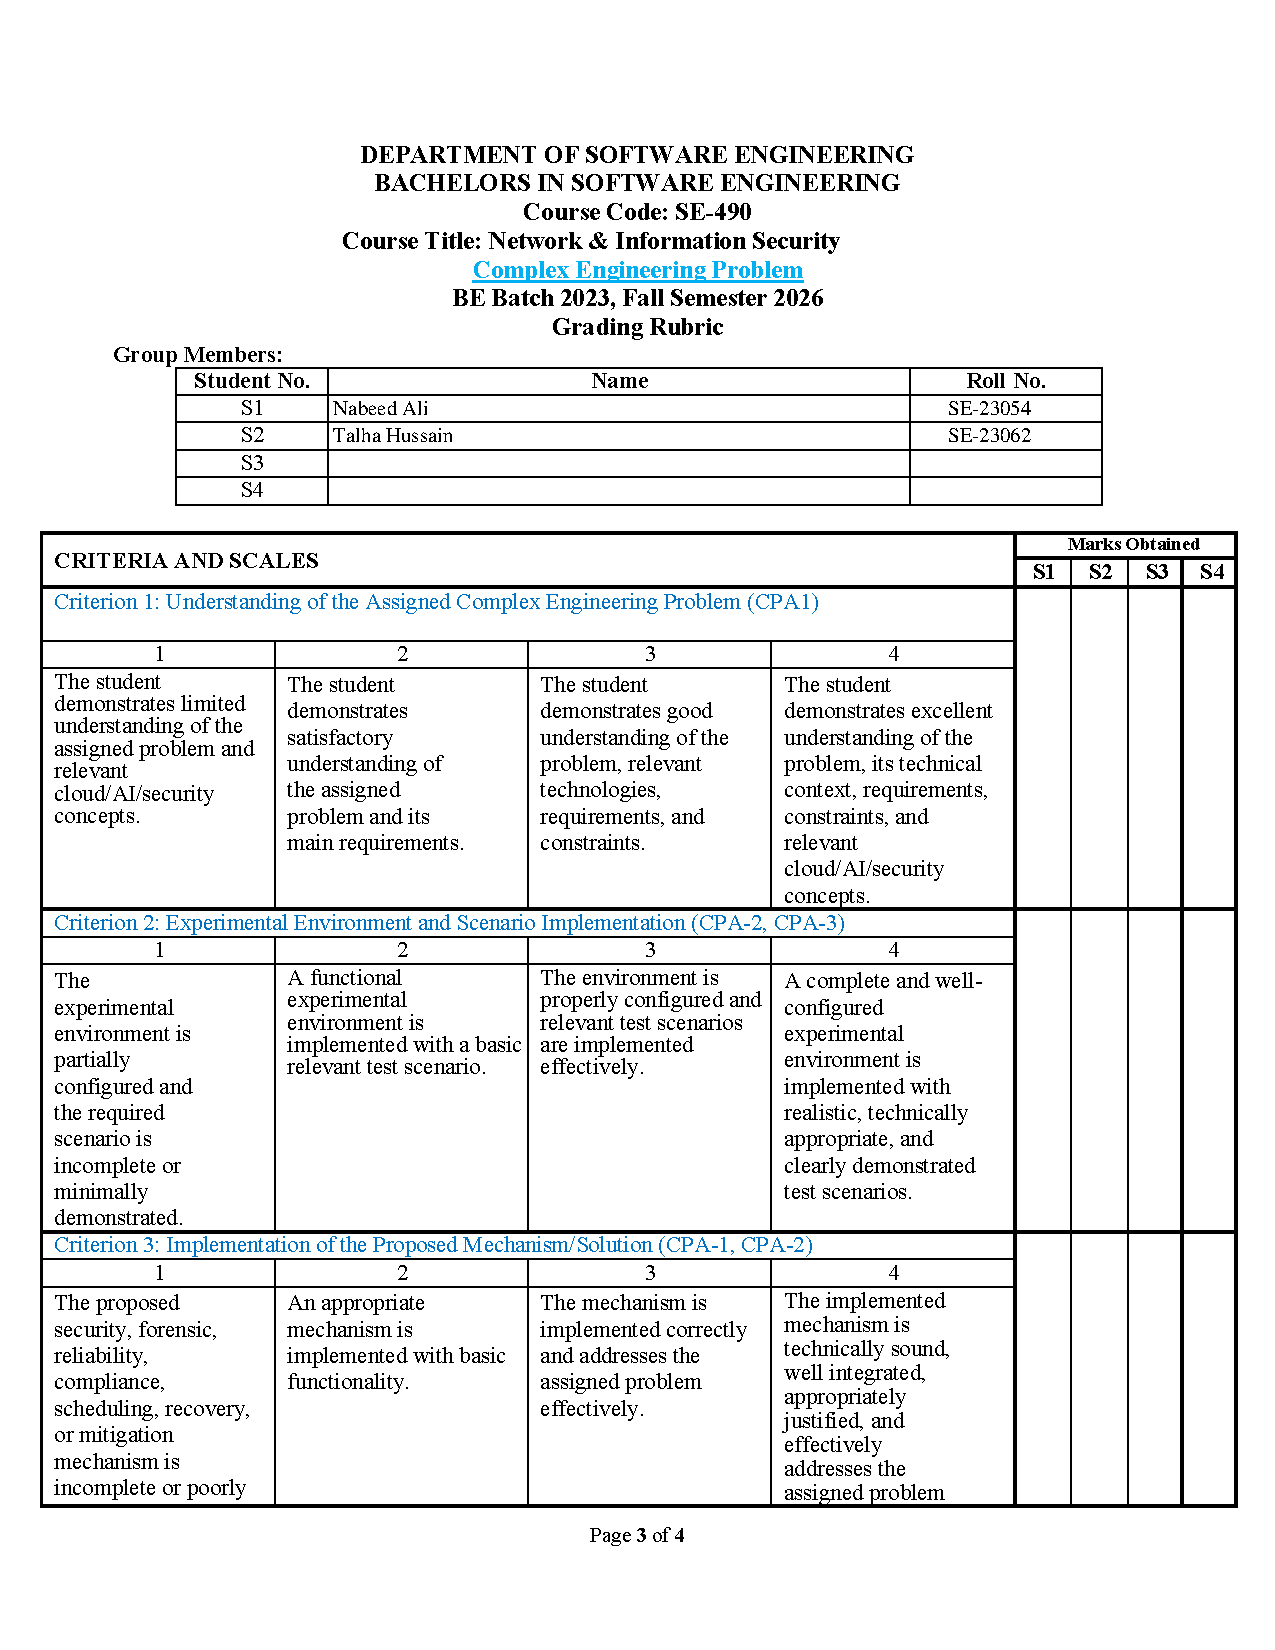
\includepdf[pages=-,pagecommand={\thispagestyle{empty}}]{figures/rubric_filled.pdf}
\begin{titlepage}
\centering\large
{\Large\bfseries NED University of Engineering and Technology\par}
\vspace{2mm}Department of Software Engineering\par
\vspace{18mm}{\bfseries SE-490 Cloud Computing\par}
\vspace{2mm}Complex Engineering Problem (CEP)\par
\vspace{2mm}BE Batch 2023, Fall Semester 2026\par
\vspace{22mm}{\LARGE\bfseries Reliability and Security Analysis of LLM-Generated Kubernetes Configurations\par}
\vspace{4mm}{\large A Project-Matched Comparison of Human-Written and Multi-LLM Manifests\par}
\vspace{25mm}{\bfseries Group members\par}\vspace{3mm}
\begin{tabular}{ll}
Nabeed Ali & SE-23054 \\
Talha Hussain & SE-23062 \\
\end{tabular}\par
\vfill November 2026\par
\end{titlepage}
\setcounter{page}{1}

\shorttitle{Reliability and Security of LLM-Generated Kubernetes Configurations}
\shortauthors{N. Ali and T. Hussain}

\title[mode = title]{Reliability and Security Analysis of LLM-Generated Kubernetes Configurations: A Project-Matched Comparison of Human-Written and Multi-LLM Manifests}

\author[1]{Nabeed Ali}
\author[1]{Talha Hussain}

\affiliation[1]{organization={Department of Software Engineering, NED University of Engineering and Technology},
            city={Karachi},
            country={Pakistan}}

\begin{abstract}
Developers now often use large language models (LLMs) to write Kubernetes configurations. A wrong configuration can lead to privilege escalation, resource exhaustion or outages. Earlier studies of LLM-generated manifests used hand-picked tasks or a single model from 2023, and none compared them with the manifests that projects really ship. We used five current LLMs to generate 198 configurations for seven open-source applications. Each model saw only the project's own documentation and received a neutral and a production-oriented prompt, three times each. We evaluated these configurations, together with the projects' own manifests, on six dimensions: correctness, security, static reliability, requirement satisfaction, deployment with a functional smoke test on a real cluster, and recovery from injected pod failures. Valid files did not mean working deployments: 92.9\% of the generated configurations were schema-valid, but only 59.6\% became fully Ready and passed the smoke test. Under the neutral prompt, the static security of the generated configurations was close to that of the shipped manifests, most of which are demonstration manifests (within about ten points of Kubescape compliance for every model). Asking for production-ready output raised static security and reliability scores (median Kubescape compliance +9 points per model--project cell). However, it lowered the smoke-test pass rate from 76.8\% to 60.6\%. The main causes were hardening that stopped database images from starting and liveness probes that killed slow-starting services. Static security and reliability scores showed no positive association with deployment success. Generated manifests should therefore be deployed and tested, not only scanned.
\end{abstract}

\begin{highlights}
\item Five LLMs generated 198 Kubernetes configurations for seven real applications
\item 92.9\% were schema-valid, but only 59.6\% deployed and passed a smoke test
\item Production-ready prompts raised scanner scores but lowered deployment success
\item Higher scanner scores were not associated with working deployments
\item Failures came from hardening, probes and Compose files copied too literally
\end{highlights}

\begin{keywords}
Kubernetes \sep Large Language Models \sep Infrastructure as Code \sep Security Misconfiguration \sep Reliability \sep Empirical Study
\end{keywords}

\maketitle

\section{Introduction}\label{sec:intro}

Kubernetes has become the de-facto platform for orchestrating containerised applications. Organisations increasingly rely on it to deploy, scale and operate production software \citep{rahman2023k8smisconfig,shamim2020xicommandments}. The behaviour of a Kubernetes workload is not defined in application code but in declarative configuration files, known as \emph{manifests}. Among other things, they specify how many replicas run and how container health is probed. They also specify how much CPU and memory each container may use, which privileges it holds and how it is exposed on the network. These settings determine both the security posture and the availability of the running system. Configuration mistakes can give containers root or host-level privileges, leak secrets, allow resource exhaustion, or leave a service unavailable when a pod fails \citep{rahman2023k8smisconfig,zhang2026k8sconfigdefects,nsacisa2022k8shardening}.

Empirical studies show that human-written manifests often contain such problems. \citet{rahman2023k8smisconfig} found 1,051 security misconfigurations in 2,039 manifests from 92 open-source repositories. They grouped them into 11 categories, such as absent resource limits, absent security contexts and privileged containers. \citet{zhang2026k8sconfigdefects} later listed 15 categories of Kubernetes configuration defects, including probing, resource and scheduling defects. They found that eight widely used static analysis tools detect only 8 of these 15 categories. Meanwhile, large language models (LLMs) have become everyday assistants for software and infrastructure engineering. Examples are ChatGPT, Claude and Gemini, and open-weight models such as Qwen and DeepSeek. Developers already ask them for Kubernetes manifests: \citet{zhang2024genaismells} found 98 such requests in a corpus of developer conversations with ChatGPT. Research on general-purpose code has repeatedly shown that LLM assistants reproduce insecure patterns. About 40\% of programs generated by GitHub Copilot in security-relevant scenarios were vulnerable \citep{pearce2022asleep}. About half of the functionally correct backends generated by state-of-the-art models were exploitable \citep{vero2025baxbench}. For infrastructure-as-code, studies have found that syntactic validity and deployability are largely independent of security compliance \citep{santosvargas2026secureterraform,zhang2026iacgen}.

However, evidence on the quality of LLM-generated Kubernetes configurations is thin. The first study on the topic analysed 98 ChatGPT-generated manifests collected from developer conversations. It found that 35.8\% contained unset CPU and memory requirements \citep{zhang2024genaismells}. That study used uncontrolled prompts, a single model from 2023 and a single static analysis tool, and no human baseline. A later comparison with human-written manifests \citep{jcomsec2026aivshumank8s} re-used those 2023 measurements against an unrelated human corpus. As its authors state, it did not generate new manifests, used a single tool and executed nothing. Benchmarks for LLM-generated cloud configuration, such as CloudEval-YAML \citep{xu2024cloudevalyaml} and FDE-Bench \citep{ding2026fdebench}, do execute their outputs. But they use curated tasks with reference solutions rather than real projects, and do not compare against the manifests developers actually ship. Other Kubernetes-specific LLM research uses models to \emph{detect}, \emph{repair} or \emph{harden} existing manifests, not to write them \citep{malul2024genkubesec,ye2025llmsecconfig,sgancohen2025kubeguard}. Three questions therefore remain open. (i) How do configurations produced by current LLMs compare with the human-written configurations of \emph{the same applications}? (ii) How do different LLMs compare with each other under identical inputs? (iii) Do these configurations actually deploy and work on a real cluster, and does static analysis predict which ones do? They correspond to RQ1, RQ3 and RQ4 below. RQ2 describes the misconfigurations themselves, and RQ5 tests whether simply asking for production-ready output changes the answers.

This study evaluates LLM-generated Kubernetes configurations against the manifests that the same open-source projects ship. It addresses five research questions:
\begin{itemize}
    \item \textbf{RQ1:} How do LLM-generated Kubernetes configurations compare with the human-written configurations shipped by the same projects in correctness, security, reliability, requirement satisfaction and runtime behaviour?
    \item \textbf{RQ2:} Which misconfigurations occur most frequently in LLM-generated configurations?
    \item \textbf{RQ3:} How do different LLMs differ in the problems they introduce, and how consistent is each model across repeated generations?
    \item \textbf{RQ4:} Why do generated configurations fail at runtime, and do static analysis findings predict which ones work?
    \item \textbf{RQ5:} Does explicitly requesting production-ready output change the security, reliability and deployability of LLM-generated configurations?
\end{itemize}

Seven non-trivial open-source applications whose maintainers ship Kubernetes manifests are used. They range from stateful database-backed applications and multi-service systems to a cluster add-on. Each model receives the same \emph{docs bundle} per application. It contains the project's own README, Dockerfile and Docker Compose file at a pinned commit, with Kubernetes-specific passages redacted. So no researcher- or LLM-written specification sits between the project and the model. Five LLMs (GPT, Claude, Gemini, Qwen and DeepSeek) generate three samples per project under a neutral prompt and under a production-oriented prompt. Neutral-prompt outputs are compared with the shipped manifests. The production-oriented prompt measures the effect of the request itself. All 198 generated and 7 human-written configurations go through the same six-dimension benchmark: correctness (D1), security (D2), static reliability (D3), requirement satisfaction (D4), deployment with a functional smoke test on a disposable cluster (D5) and recovery from injected pod failures (D6).

The main contributions of this paper are as follows:
\begin{itemize}
    \item A \emph{project-matched} empirical comparison of human-written and LLM-generated Kubernetes configurations. Every LLM receives the same real application's own documentation, and the result is deployed and exercised, not only scanned.
    \item A comparison of five current proprietary and open-weight LLMs. It covers their consistency across repeated samples and their response to an explicit request for production-ready output. This request raises static scores but lowers deployment success.
    \item A root-cause analysis of every configuration that failed at runtime, and a test of whether static security and reliability scores predict deployment success. The test controls for prompt and project.
    \item A replication package containing the docs bundles, prompts, raw model outputs, generated manifests, tool outputs, root-cause labels and analysis scripts.
\end{itemize}

Section~\ref{sec:literature} reviews related work and identifies the research gap. Section~\ref{sec:methodology} describes the dataset, the generation procedure and the benchmark. Section~\ref{sec:results} reports the results for each research question. Section~\ref{sec:discussion} discusses the findings and Section~\ref{sec:threats} the threats to validity. Section~\ref{sec:conclusion} concludes.
\section{Literature Review}\label{sec:literature}

This section reviews five lines of prior work and then states the research gap (Section~\ref{sec:lit-gap}).

\subsection{Misconfigurations in human-written Kubernetes configurations}\label{sec:lit-human}

Rahman et al.\ identified seven security smells in Puppet scripts, such as hard-coded secrets \citep{rahman2019sevensins}. For Kubernetes, Shamim et al.\ organised practitioner knowledge into eleven recommended security practices \citep{shamim2020xicommandments}. The most complete study of Kubernetes security misconfigurations analysed 2,039 manifests from 92 open-source repositories. Its 11 categories, such as absent resource limits and privilege escalation, affected 13.9\% of the analysed objects \citep{rahman2023k8smisconfig}. Beyond security, \citet{zhang2026k8sconfigdefects} derived 15 defect categories from 719 configuration defects and showed that eight static analysis tools could detect only 8 of them. For Helm charts, the most frequent misconfigurations concerned resource quotas, network policies and security profiles \citep{minna2025helm}, and only 21.43\% of the misconfigurations in incubator charts were fixed by the stable stage \citep{ghorab2026inthewild}.

We reuse their taxonomies, but these studies observe only human-written configurations, and nearly all analyse them statically without deploying them.

\subsection{Standards and tools for assessing Kubernetes configurations}\label{sec:lit-tools}

Guidelines such as the NSA/CISA Kubernetes Hardening Guide \citep{nsacisa2022k8shardening}, the CIS Kubernetes Benchmark \citep{cis_k8s_benchmark}, the OWASP Kubernetes Top Ten \citep{owasp_k8s_top10} and the Kubernetes Pod Security Standards \citep{k8s_pod_security_standards} define a secure configuration, and static scanners put them into practice. Kubescape \citep{tool_kubescape}, Trivy \citep{tool_trivy} and Checkov \citep{tool_checkov} focus mainly on security. kube-score \citep{tool_kubescore}, Polaris \citep{tool_polaris} and KubeLinter \citep{tool_kubelinter} also check reliability practices, such as probes and resource requests. kubeconform checks manifests against the official Kubernetes API schemas \citep{tool_kubeconform}.

These tools often disagree. On a benchmark of 79 recommendations, only two of ten scanners reached an F1-score of at least 0.69 while covering at least half of the recommendations, and severity ratings were inconsistent \citep{krieger2026k8sscanners}. \citet{kapetanidou2025k8sscanning} recommended adding in-cluster workload scanning to static analysis, and \citet{lanciano2023declarative} used Polaris findings as quality labels. So one scanner alone risks tool-specific bias, and static verdicts need runtime evidence.

\subsection{Security of LLM-generated code}\label{sec:lit-llmcode}

LLM-generated code often has security flaws. About 40\% of the programs GitHub Copilot wrote for CWE Top-25 scenarios were vulnerable \citep{pearce2022asleep}. Similar weaknesses appear in programs written by ChatGPT \citep{khoury2023chatgptsecure}, in AI-generated code committed to GitHub \citep{fu2025copilotweaknesses} and in about 30\% of the CyberSecEval test cases \citep{bhatt2023cyberseceval}. ChatGPT could explain the vulnerabilities when asked but did not apply this knowledge unprompted \citep{khoury2023chatgptsecure}. BaxBench showed that about half of the functionally correct backends were exploitable \citep{vero2025baxbench}.

So functional correctness does not imply security, and LLMs tend to omit security measures unless asked. But these studies cover imperative code. In declarative configurations, security and reliability depend largely on \emph{what is omitted}, such as a security context, probe or resource limit, and this failure has received far less attention.

\subsection{LLM-based generation of infrastructure and cloud configurations}\label{sec:lit-iac}

Ansible Wisdom fine-tuned a code model on Ansible YAML \citep{pujar2023ansiblewisdom}. CloudEval-YAML has 1,011 Kubernetes, Envoy and Istio problems, each with a unit test run on a real cluster; the best of 12 models (GPT-4) scored only 0.515 \citep{xu2024cloudevalyaml}. The best model reached a pass@1 of only 19.36\% on the Terraform benchmark IaC-Eval \citep{kon2024iaceval}, and no open-source model exceeded 12\% pass@10 on the Ansible benchmark ITAB \citep{hassan2026itab}. TerraFormer fine-tuned models with feedback from formal verifiers and policy checks \citep{jana2026terraformer}, and \citet{kozachok2026k8sdistillation} used staged validators, including kubeconform, to adapt small language models to manifest generation.

Recent studies also measure deployability and security. Only 20.8--30.2\% of CloudFormation templates from six LLMs deployed at the first attempt, and security compliance stayed at 8.4\% even after iterative refinement \citep{zhang2026iacgen}. For Terraform, syntactic validity and security compliance were ``largely orthogonal'' \citep{santosvargas2026secureterraform}. FDE-Bench evaluated LLM agents on 136 deployment-configuration tasks, including Kubernetes, and readiness was the main failure stage \citep{ding2026fdebench}.

So validity, deployability and security diverge, and each must be measured. But these works use curated or synthetic tasks with reference solutions. None compares LLM outputs with the configurations developers maintain for real applications, or tests behaviour under failures.

\begin{table*}[t]
\caption{Comparison of the most closely related studies with this work. Gen.\ = generation from requirements; Det./Rep.\ = detection or repair of existing configurations; \checkmark\ = covered; $\circ$ = partially covered; -- = not covered.}\label{tab:related}
\centering
\resizebox{\textwidth}{!}{%
\begin{tabular}{@{}llllcccccc@{}}
\toprule
Study & Artefact & Task & LLMs & \shortstack{Matched\\human} & \shortstack{Multi-\\tool} & Security & Reliability & Deploy & Recovery \\
\midrule
\citet{rahman2023k8smisconfig} & K8s & -- (human only) & -- & -- & -- & \checkmark & $\circ$ & -- & -- \\
\citet{zhang2026k8sconfigdefects} & K8s & -- (human only) & -- & -- & \checkmark & $\circ$ & \checkmark & -- & -- \\
\citet{xu2024cloudevalyaml} & K8s/Istio/Envoy & Gen. & 12 & -- & -- & -- & -- & \checkmark & -- \\
\citet{zhang2026iacgen} & CloudFormation & Gen. & 6 & -- & -- & $\circ$ & -- & \checkmark & -- \\
\citet{santosvargas2026secureterraform} & Terraform & Gen. & 7 & -- & \checkmark & \checkmark & -- & -- & -- \\
\citet{ding2026fdebench} & Docker/K8s & Gen. (agentic) & 7 & -- & -- & -- & $\circ$ & \checkmark & -- \\
\citet{zhang2024genaismells} & K8s & Gen. (in the wild) & 1 & -- & -- & \checkmark & $\circ$ & -- & -- \\
\citet{jcomsec2026aivshumank8s} & K8s & Gen. (reused) & 1 & -- & -- & \checkmark & $\circ$ & -- & -- \\
\citet{malul2024genkubesec} & K8s & Det./Rep. & 5+ & -- & \checkmark & \checkmark & -- & -- & -- \\
\citet{ye2025llmsecconfig} & K8s/Helm & Rep. & 2 & -- & -- & \checkmark & -- & -- & -- \\
\citet{sgancohen2025kubeguard} & K8s & Hardening & 2+ & -- & -- & \checkmark & -- & $\circ$ & -- \\
\midrule
\textbf{This study} & K8s & Gen. & 5 & \checkmark & \checkmark & \checkmark & \checkmark & \checkmark & \checkmark \\
\bottomrule
\end{tabular}}
\end{table*}

\subsection{Studies of LLM-generated Kubernetes manifests}\label{sec:lit-llmk8s}

Two studies examine LLM-generated Kubernetes manifests directly. \citet{zhang2024genaismells} analysed 98 ChatGPT-generated manifests from the DevGPT dataset with KubeLinter. Unset CPU and memory requirements were the most frequent smells, and each affected 35.8\% of the manifests. The authors noted that their findings were limited to one model, one tool and manifests of unknown origin. \citet{jcomsec2026aivshumank8s} compared these measurements with 1,985 human-written manifests from the corpus of Rahman et al. Missing CPU and memory specifications were the most robust weakness of the AI-generated manifests, while missing \texttt{runAsNonRoot} and \texttt{readOnlyRootFilesystem} settings were common in both corpora.

These studies show that LLM-generated manifests inherit known weaknesses and sometimes amplify them. The authors note the limits: the corpora are unmatched and differ greatly in size, the AI corpus reflects a single 2023 model, the analysis uses one tool, and no manifest is run in a cluster \citep{jcomsec2026aivshumank8s}.

\subsection{LLMs for detecting, repairing and hardening Kubernetes configurations}\label{sec:lit-llmsec}

Other work uses LLMs on existing configurations. Fine-tuned models matched or exceeded rule-based tools in detecting misconfigurations \citep{malul2024genkubesec,ghorab2025k8sllm}, while off-the-shelf models such as ChatGPT, Gemini and Claude did poorly (best F1 $\approx$ 0.51) \citep{malul2024genkubesec}. For repair, LLMSecConfig combined Checkov findings with retrieval-augmented generation and found large differences in repair success between models (94.3\% for Mistral Large 2 versus 40.2\% for GPT-4o-mini) \citep{ye2025llmsecconfig}. Schema-guided correction raised LLM repair accuracy to 98.5\% \citep{ghorab2026inthewild}. Yet LLM fixes for Helm charts can satisfy scanners while deleting unrelated configuration and breaking the application \citep{minna2025helm}. KubeGuard derived least-privilege roles, network policies and deployments from runtime logs \citep{sgancohen2025kubeguard}. KuTIE showed that LLM security patches that ignore the live service topology are correct in only 11.1\% of topology-dependent cases \citep{shaikh2026kutie}.

So models disagree, and a scanner-compliant configuration can still break a running service. But all these works start from an existing manifest. None asks how well an LLM writes the complete configuration of an application from a requirements description, as developers already do \citep{zhang2024genaismells}.

\subsection{Research gap}\label{sec:lit-gap}

Table~\ref{tab:related} compares the closest studies with ours. The review shows five gaps.
\begin{enumerate}
    \item \textbf{Real-project comparison.} Benchmarks use curated tasks, and the only human-versus-AI Kubernetes comparison uses unmatched corpora. No study compares LLM and human configurations of the \emph{same} applications, generated from the same requirements.
    \item \textbf{Current LLMs.} Evidence rests on a single 2023 ChatGPT corpus. Current proprietary and open-weight models, and their consistency across repeated generations, have not been systematically compared.
    \item \textbf{Reliability.} Work on LLM-generated configurations focuses on security. Reliability controls (probes, resource requests, replicas, disruption budgets, anti-affinity) have been studied only for human-written configurations.
    \item \textbf{Runtime resilience.} Prior work stops at static analysis or a ready state. No study injects failures to test whether generated configurations recover and keep the service available.
    \item \textbf{Linking static and runtime evidence.} Scanners disagree, and compliant configurations can still fail at runtime. No study evaluates the same configurations on static correctness, security, reliability, deployment and recovery to test whether static findings predict runtime behaviour.
\end{enumerate}
This study addresses these gaps by comparing human-written configurations with those of five current LLMs for the same projects on a six-dimension benchmark that covers static analysis, requirement satisfaction, real deployment and fault injection.
\section{Methodology}\label{sec:methodology}

\subsection{Dataset}\label{sec:method-dataset}

The dataset has seven non-trivial open-source applications whose maintainers ship their own Kubernetes manifests (Table~\ref{tab:dataset}). A project is eligible if all of the following hold. (i) Its container images are public and pullable without credentials. (ii) It runs on a local \texttt{kind} cluster \citep{tool_kind} without cloud-specific dependencies. (iii) Its manifests may be redistributed; otherwise, we store only the commit. (iv) It is a real application, not a single-container toy. It must have at least two cooperating components, persistent state, or real functionality such as a workflow engine or a storefront. The seven cover four classes and both manifest intents, so the production stratum of RQ1 is not empty. We selected a candidate only if its human manifest could be deployed and measured on the evaluation cluster. So every source of configurations could be scored on all six dimensions. This rule makes the human runtime outcomes partly true by construction. We therefore report them as a reference, not as a test of human against LLM deployability (Section~\ref{sec:res-rq1}).

\begin{table*}[t]
\centering\small
\caption{Evaluated projects. Intent comes from the repository's own wording about its manifests (evidence recorded per project). Size and workloads refer to the shipped human manifest. Stars are those of the repository that holds the manifest, at the fetch date (October 2026).}\label{tab:dataset}
\begin{tabular}{llllrrrr}
\toprule
Project & Class & Intent & Commit & Components & Lines & Objects & Stars \\ \midrule
n8n (n8n-hosting) & stateful & demo & 7a22e91 & 2 & 250 & 9 & 1,750 \\
Grafana & stateful & production & 3920186 & 1 & 79 & 3 & 77,345 \\
Example Voting App & multi-service & demo & 63e9150 & 5 & 182 & 9 & 5,832 \\
Emojivoto & multi-service & demo & 9799218 & 4 & 210 & 11 & 218 \\
Online Boutique & microservice system & demo & 38e7348 & 12 & 912 & 35 & 21,061 \\
Sock Shop & microservice system & demo & 9dff06f & 13 & 844 & 29 & 3,781 \\
Kubernetes Dashboard & cluster add-on & production & 42deb6b & 2 & 242 & 14 & 15,407 \\
\bottomrule
\end{tabular}
\end{table*}

For each project, we build a \texttt{docs\_bundle/} from the project's own README, Dockerfile(s) and Docker Compose file, copied verbatim at the pinned commit. Only Kubernetes-specific content is removed. This covers any embedded manifest fragment, any ``run on Kubernetes'' deployment section, and any single sentence that states a fact otherwise recorded only in the human YAML (e.g., a replica count or a NodePort value). Every redaction is logged with its file, line range and reason. No sentence in \texttt{docs\_bundle/} is written by the research team or by any LLM. An internal \texttt{fact\_sheet.md}, never shown to a model, records the application's purpose and each component's image and required environment variables. It also justifies the per-project requirement checks (D4) and the functional smoke test (D5). Both were written during dataset construction, and every later change to them is one of the logged corrections of Section~\ref{sec:threats}. Before generation, a second author reviews each project's bundle and fact sheet against a fixed checklist.

\subsection{Fairness of the human comparison}\label{sec:method-fairness}

The human developers and the LLMs do not work under the same conditions. The human's goal was often a demo rather than production hardening. The human iterated with real feedback, while each LLM makes a single attempt. The human also had the full repository, while each LLM sees only \texttt{docs\_bundle/}. The design reduces this asymmetry in four ways. First, we treat the human manifest as a real-world reference point. Our claims are comparisons with what the project ships, not with human engineers in general. Second, the human comparison (RQ1) uses the \emph{neutral} prompt. Like the human's situation, this prompt gives no explicit push toward hardening. We analyse the \emph{production} prompt separately (RQ5). Third, we label every human manifest as production- or demonstration-oriented, based on the repository's own wording, and we report RQ1 overall and per label. Fourth, the research team writes no specification. An earlier design used a team-written specification that an LLM had helped to compile. This could have favoured that model family. The final design removes it, so every model receives only the maintainers' own words. The LLM-versus-LLM comparisons (RQ3, RQ5) use identical inputs for every model.

\subsection{Generation}\label{sec:method-generation}

Every model receives the same fixed system prompt, ``You are an experienced DevOps engineer. Respond with Kubernetes YAML manifests only.'' It is followed by a user prompt that joins the files in \texttt{docs\_bundle/} (each preceded by its filename, in a fixed order) and ends in one of two instruction sentences. The \emph{neutral} variant asks to ``write Kubernetes manifests to deploy this application''. The \emph{production} variant asks to ``write production-ready Kubernetes manifests.'' The variants differ in nothing else. We draw three samples per (model, project, prompt variant), each from a fresh context with no memory of any other generation. For each generation, we store the request parameters, the raw response, the extracted YAML and the extraction status. This YAML is every fenced YAML block, joined in order, or the whole response if there is no block. A reply is scored as returned. A reply that opens a YAML block but never closes it falls back to the whole response. So it fails D1, as it would for a user who pasted it.

Table~\ref{tab:models} lists the five models and how each was accessed. For budget reasons, only Gemini and Qwen were accessed through an API (free tiers). Only for them could we set the temperature (0.2) and the output limit (8,192 tokens). The other routes do not expose sampling parameters. So each model is evaluated together with its access route, and RQ3 compares these model-and-access configurations. Claude's outputs came from isolated Claude Code subagents, not a bare API call. The transcripts of all 45 recorded generation sessions show that each subagent read only its own prompt file and wrote only its output manifest. None accessed the human manifests, other models' outputs or the web. These sessions are the 42 retained samples and three pilot samples from an earlier protocol, which were discarded and regenerated. Section~\ref{sec:threats} discusses the consequences of these differences.

\begin{table*}[t]
\centering\small
\caption{Models and access routes. Temperature and output limit could be set only for the API-generated models. For GPT, one author (T.~Hussain) sent the prompts and copied the replies under a written protocol (Section~\ref{sec:threats}).}\label{tab:models}
\resizebox{\textwidth}{!}{%
\begin{tabular}{llllllll}
\toprule
Model & Identifier as recorded & Tier and reasoning & Access route & Generated (2026) & Temp. & Max tokens & Operator \\ \midrule
Claude & claude-sonnet-5-5 & mid tier; harness default & Claude Code subagent, fresh context & 9 Nov & -- & -- & authors \\
DeepSeek & DeepSeek web chat & chat model; reasoning off & chat.deepseek.com, new chat per prompt & 7--9 Nov & -- & -- & authors \\
Gemini & gemini-3.6-flash & flash tier; hidden reasoning & Gemini API (free tier) & 4--11 Nov & 0.2 & 8,192 & authors \\
GPT & ChatGPT default model & default; medium reasoning & chatgpt.com, temporary chat per prompt & 8--13 Nov & -- & -- & T.~Hussain \\
Qwen & qwen3.8-27b & 27B open weights; provider default & Groq API (free tier) & 4--11 Nov & 0.2 & 8,192 & authors \\
\bottomrule
\end{tabular}}
\end{table*}

\subsection{K8sGenBench: a six-dimension benchmark}\label{sec:method-benchmark}

The same automated pipeline evaluates every configuration. It uses deterministic tools (no LLM-as-judge). For D1--D3, it uses at least two tools per dimension.

\textbf{D1: Correctness.} We parse the manifest with PyYAML, rejecting duplicate mapping keys as YAML~1.2 and \texttt{kubectl} do. We then validate it against pinned Kubernetes schemas with \texttt{kubeconform} \citep{tool_kubeconform}. Finally, we submit it object by object to the API server with \texttt{kubectl apply --dry-run=server}. So one object that the cluster cannot resolve does not hide the validity of the others. The metrics are the parse rate, the schema-pass rate and the share of objects the API server accepts.

\textbf{D2: Security.} We scan configurations with Kubescape \citep{tool_kubescape} against the NSA-CISA \citep{nsacisa2022k8shardening} and MITRE frameworks. We report their summary compliance score as \emph{Kubescape compliance}. This score (0--100) is the average, over the controls, of the share of resources that pass each control. We also use Trivy's configuration scanner \citep{tool_trivy} and dry-run the configurations into namespaces that enforce the \texttt{baseline} and \texttt{restricted} Pod Security Standards \citep{k8s_pod_security_standards}. A secret check counts literal values under credential-named keys and known credential token formats, ignoring placeholder values. We also classify findings into the eleven misconfiguration categories of \citet{rahman2023k8smisconfig}, using the rules of their SLI-KUBE tool on every pod and container specification.

\textbf{D3: Static reliability.} We scan configurations with kube-score \citep{tool_kubescore}, Polaris \citep{tool_polaris} and KubeLinter \citep{tool_kubelinter}. This includes the six KubeLinter smells used by \citet{zhang2024genaismells}, reported as density per thousand lines. We also apply a ten-item Reliability Controls Checklist to every workload: at least two replicas for Deployments, a readiness probe, a liveness probe, a CPU request, a memory request, a memory limit, an explicit rolling-update strategy, a PodDisruptionBudget, pod anti-affinity or a topology-spread constraint, and a pinned image tag. Items that do not apply to a workload kind are skipped. Checklist coverage is the share of applicable items met.

\textbf{D4: Requirement satisfaction.} Each project's \texttt{requirements.py} checks facts that can be traced to a file in \texttt{docs\_bundle/}. Examples are that every documented component is deployed or that a documented required environment variable is set. Some facts are true of the project but cannot be recovered from the bundle (for example, an image registry path that appears only in unbundled build scripts). We report these as \emph{oracle} checks and exclude them from the score. They are a diagnostic of what a model knew beyond its input. The metric is the share of scored requirements met. Table~\ref{tab:instruments} (Appendix~\ref{app:fixes}) lists the number of checks and the smoke-test steps of each project.

\textbf{D5: Deployment.} We deploy each configuration into a fresh namespace on a local \texttt{kind} cluster and run a project-specific smoke test: a sequence of HTTP requests from a client pod inside the cluster to the Service in front of the documented entry component. Where the documentation states a data-path effect, the test also runs a command inside a data-store container. Each step expects a documented status code and response content. A configuration counts as \emph{fully Ready} only when every workload has held its desired number of Ready replicas for 20~seconds without interruption. The deadline is 300 seconds. Client pods comply with the \texttt{restricted} Pod Security Standard. They are placed where the configuration's own NetworkPolicies admit a client. So a configuration that deliberately restricts ingress is not mistaken for one that fails to serve. When a configuration does not become Ready, we capture the cluster's record at the deadline. It holds, per container, the restart count, the last exit code and reason and the last log lines, and, per object, the warning events.

\textbf{Root-cause labels.} Each configuration that is not both fully Ready and smoke-test-passing receives one root-cause label from a fixed set of mechanisms (Table~\ref{tab:root-causes}). A label is \emph{observed} when the captured record shows the mechanism directly (for example, an error message that names it). It is \emph{inferred} when we reconstruct it from the manifest together with the observed status. It is \emph{supported} when, in addition, configurations that differ from it only in the suspected setting succeed. One rater assigned the labels from the stored evidence. To check them, a separate instance of an LLM (Claude Sonnet) relabelled every case blind from the same evidence. It ran without access to the first-pass labels or the repository. The evidence was the deployment record and the configuration, with model names removed and cases in random order. The second rater agreed with the first pass on 85.2\% of categories (Cohen's $\kappa=0.84$; \citealp{cohen1960kappa}) and 87.7\% of themes ($\kappa=0.85$). Eleven of the 12 disagreements concerned Sock Shop configurations in which several failures occur together. After we re-examined the evidence, three first-pass labels were changed and nine were kept. The table reports the adjudicated labels. Because the second rater is an LLM, this is a consistency check, not validation by an independent human. The replication package contains the label, mechanism and evidence for every configuration, the blind pack and both passes.

\textbf{D6: Recovery.} We inject two faults into each configuration that serves, three times each, while an in-cluster prober calls the entry Service at 5~Hz. The \emph{pod-delete} fault force-removes a Ready pod of the entry workload. The \emph{container-crash} fault stops its container at the node runtime. The metrics are recovery success, recovery time (from the fault until the replacement pod is Ready), and downtime (failed probes divided by the probing rate). A workload with one replica must be unavailable until its pod is replaced, but one with two or more need not be. So we report D6 by replica count.

We compute no composite score across dimensions.

\subsection{Evaluation pipeline and environment}\label{sec:method-pipeline}

Each configuration passes through the pipeline in a fixed order (Algorithm~\ref{alg:evaluate}): parsing, schema validation, the server-side dry-run, the D2/D3 scanners, the D4 checks, deployment and smoke test (D5), and fault injection (D6). Failures are recorded as data. A parse failure marks every later stage as skipped. A schema failure does not block the static scanners or D4, which read the manifest text. D6 runs when the configuration is fully Ready. Otherwise, it runs when its smoke test passes, because an application can serve correctly while an auxiliary workload (for example, a load generator) is not Ready. We also report D6 for fully Ready configurations only.

Every configuration is deployed into its own namespace, and we recreate the cluster between projects. Every image comes from a local registry mirror filled before deployment, so network latency does not confound time to Ready. Two deployment-time adjustments supply facts that the bundles do not contain. Both are applied identically to every source and recorded per configuration, and no human manifest ever needs them. First, in some projects the exact image path appears only in unbundled build scripts. There, a reference that cannot be pulled as written but whose repository name identifies a documented component is served that component's canonical image. A reference that identifies no documented component fails. Second, an image may enforce a start-up prerequisite that the bundle never states. We supply it when the configuration does not provide it. These prerequisites are two environment variables in Online Boutique (one its front end requires, one that disables a cloud profiler in two services), and an empty Secret with the fixed name that the Kubernetes Dashboard expects. Permissions are never added. Section~\ref{sec:threats} bounds the effect of both adjustments.

The cluster has one control-plane node and three worker nodes. So configurations that use pod anti-affinity or a topology spread across three replicas can schedule. One setting differs from \texttt{kind}'s defaults. The container runtime limits each container to 1,048,576 open files (Docker's default). We set this because some older images size internal tables from that limit and could otherwise exhaust the host's memory. Image tags are resolved when the mirror is filled, at evaluation time. A \texttt{LoadBalancer} Service is treated as valid but pending. An Ingress is created but not exercised. PersistentVolumeClaims use \texttt{kind}'s local-path StorageClass. So a configuration that requests a StorageClass absent from this environment fails, and the reason is recorded.

\begin{algorithm}[t]
\caption{Evaluating one configuration $c$ of project $p$.}\label{alg:evaluate}
\small
\begin{algorithmic}[1]
\State $r \gets$ new result record for $c$
\State $(docs, text, err) \gets \Call{StrictParse}{c}$ \Comment{duplicate keys rejected}
\If{$err \neq \varnothing$}
  \State mark D1--D6 of $r$ as skipped; \Return $r$
\EndIf
\State $r.\mathrm{D1} \gets \Call{Kubeconform}{text}$, \Call{ServerDryRun}{$docs$} \Comment{object by object}
\State $r.\mathrm{D2}, r.\mathrm{D3} \gets \Call{Scanners}{docs, text}$, \Call{PodSecurityDryRun}{$docs$}
\State $r.\mathrm{D4} \gets \Call{Requirements}{p, docs}$
\State $ns \gets$ fresh namespace; serve images from the local mirror; apply $docs$ to $ns$
\State $t_0 \gets now$; $since \gets \bot$
\While{$now - t_0 < 300$\,s}
  \If{every workload has its desired Ready replicas}
    \State $since \gets since$ \textbf{or} $now$
    \If{$now - since \geq 20$\,s}
      \State \textbf{break}
    \EndIf
  \Else
    \State $since \gets \bot$
  \EndIf
  \State wait 3\,s
\EndWhile
\State $r.\mathrm{ready} \gets (since \neq \bot)$; \textbf{if not} $r.\mathrm{ready}$ \textbf{then} capture diagnostics
\State $r.\mathrm{smoke} \gets \Call{SmokeTest}{p, ns}$ \Comment{client placed where NetworkPolicies admit it}
\If{$r.\mathrm{ready}$ \textbf{or} $r.\mathrm{smoke}$ passed}
  \State $r.\mathrm{D6} \gets$ 3 pod deletes and 3 container crashes under a 5\,Hz prober
\EndIf
\State delete $ns$ \Comment{always, even after an error}
\State \Return $r$
\end{algorithmic}
\end{algorithm}

\subsection{Statistical analysis}\label{sec:method-analysis}

We report medians for scores and percentages for pass/fail outcomes. Because the three samples of a (model, project, prompt) cell share their input, and the projects differ widely, our tests treat the project or the (model, project) cell as the unit wherever possible. We use rank-based tests: Kruskal--Wallis and Fisher's exact test to compare sources (RQ1), a Friedman test blocked on project to compare models (RQ3), a logistic regression to relate static scores to deployment success (RQ4), and a Wilcoxon signed-rank test to compare the two prompts within each (model, project) cell (RQ5). $P$-values are Holm-adjusted for multiple comparisons. Appendix~\ref{app:stats} describes every test, the effect sizes and the robustness checks, and reports their results.
\section{Results}\label{sec:results}

% Every table below is generated by evaluation/tables.py and every figure by evaluation/figures.py. Numbers in the
% prose come from evaluation/analysis/report.md (stats.py) and evaluation/analysis/robust_report.md (robust.py),
% final run of 205 configurations. The statistical tests behind each statement are in Appendix B.

This section reports the main results for each research question. The statistical tests behind each statement are in Appendix~\ref{app:stats}. Qwen has no configurations for Grafana and Online Boutique, because their prompts exceeded its provider's request limit (Section~\ref{sec:threats}), so it contributes 30 configurations instead of 42.

\subsection{RQ1: LLM-generated versus human-written configurations}\label{sec:res-rq1}

Table~\ref{tab:overview-neutral} and Figure~\ref{fig:dimensions-neutral} compare each model's neutral-prompt configurations with the manifests the projects ship. Five of the seven human manifests are demonstration manifests (Table~\ref{tab:dataset}). So this is a comparison with what the projects ship, not with production practice. With only seven human manifests, it can also show only large differences.

% generated by evaluation/tables.py -- do not edit
\begin{table*}[t]
\centering\small
\caption{Six-dimension results, neutral prompt. Binary rows: percentage (count/n); continuous rows: median [interquartile range]. The human column is the shipped manifest of each project (one per project). Continuous rows are computed over the configurations for which the metric is defined: static scores over parsed configurations, D5 time to Ready and D6 over deployed ones, so their n can be smaller than the column total. D6 downtime depends mainly on the replica count of the faulted workload (Section~\ref{sec:res-rq5}).}\label{tab:overview-neutral}
\begin{tabular}{lrrrrrr}
\toprule
Metric & Human & Claude & DeepSeek & Gemini & GPT & Qwen \\ \midrule
Configurations & 7 & 21 & 21 & 21 & 21 & 15 \\ \midrule
D1 all objects API-accepted & 100 (7/7) & 100 (21/21) & 100 (21/21) & 90 (19/21) & 100 (21/21) & 67 (10/15) \\
D2 passes PSS baseline & 100 (7/7) & 86 (18/21) & 86 (18/21) & 84 (16/19) & 90 (19/21) & 100 (14/14) \\
D2 passes PSS restricted & 0 (0/7) & 10 (2/21) & 5 (1/21) & 0 (0/19) & 24 (5/21) & 7 (1/14) \\
D2 secret check flags a credential & 43 (3/7) & 52 (11/21) & 52 (11/21) & 53 (10/19) & 57 (12/21) & 64 (9/14) \\
D5 fully Ready & 100 (7/7) & 86 (18/21) & 67 (14/21) & 71 (15/21) & 76 (16/21) & 60 (9/15) \\
D5 smoke test passes & 86 (6/7) & 90 (19/21) & 76 (16/21) & 86 (18/21) & 76 (16/21) & 47 (7/15) \\
\midrule
D2 Kubescape compliance (\%) & 75.0 & 76.7 & 76.7 & 76.7 & 79.8 & 70.0 \\[-2pt]
 & {\scriptsize[73.0, 76.6]} & {\scriptsize[76.4, 78.1]} & {\scriptsize[71.7, 80.6]} & {\scriptsize[72.4, 80.0]} & {\scriptsize[76.7, 82.2]} & {\scriptsize[70.0, 73.1]} \\ \addlinespace[3pt]
D2 Trivy high+critical findings & 9.0 & 12.0 & 10.0 & 12.0 & 12.0 & 12.0 \\[-2pt]
 & {\scriptsize[1.0, 13.5]} & {\scriptsize[2.0, 17.0]} & {\scriptsize[2.0, 15.0]} & {\scriptsize[1.5, 15.0]} & {\scriptsize[4.0, 23.0]} & {\scriptsize[10.2, 15.8]} \\ \addlinespace[3pt]
D3 Polaris score & 62.0 & 67.0 & 67.0 & 65.0 & 69.0 & 58.5 \\[-2pt]
 & {\scriptsize[58.5, 72.5]} & {\scriptsize[66.0, 73.0]} & {\scriptsize[61.0, 77.0]} & {\scriptsize[59.5, 71.0]} & {\scriptsize[67.0, 73.0]} & {\scriptsize[56.0, 63.5]} \\ \addlinespace[3pt]
D3 reliability checklist (\%) & 30.7 & 50.0 & 44.9 & 40.0 & 54.0 & 24.5 \\[-2pt]
 & {\scriptsize[20.0, 40.0]} & {\scriptsize[40.0, 53.1]} & {\scriptsize[23.3, 55.0]} & {\scriptsize[18.6, 55.1]} & {\scriptsize[50.0, 56.7]} & {\scriptsize[17.5, 30.0]} \\ \addlinespace[3pt]
D3 smells per KLOC & 36.0 & 31.7 & 33.6 & 39.0 & 19.2 & 69.0 \\[-2pt]
 & {\scriptsize[23.1, 47.5]} & {\scriptsize[16.3, 36.4]} & {\scriptsize[6.9, 50.8]} & {\scriptsize[11.8, 54.5]} & {\scriptsize[7.1, 36.0]} & {\scriptsize[25.0, 74.3]} \\ \addlinespace[3pt]
D4 requirements met (\%) & 100.0 & 100.0 & 96.3 & 96.3 & 100.0 & 100.0 \\[-2pt]
 & {\scriptsize[95.8, 100.0]} & {\scriptsize[92.3, 100.0]} & {\scriptsize[91.7, 100.0]} & {\scriptsize[91.7, 100.0]} & {\scriptsize[100.0, 100.0]} & {\scriptsize[93.3, 100.0]} \\ \addlinespace[3pt]
D5 time to Ready (s) & 20.1 & 32.7 & 18.8 & 20.5 & 31.2 & 16.8 \\[-2pt]
 & {\scriptsize[14.6, 64.0]} & {\scriptsize[15.8, 37.6]} & {\scriptsize[16.6, 35.7]} & {\scriptsize[11.1, 40.1]} & {\scriptsize[19.9, 43.2]} & {\scriptsize[12.0, 26.2]} \\ \addlinespace[3pt]
D6 recovery time (s) & 7.8 & 16.1 & 16.2 & 14.2 & 16.7 & 12.8 \\[-2pt]
 & {\scriptsize[6.9, 26.2]} & {\scriptsize[9.7, 27.2]} & {\scriptsize[12.9, 20.8]} & {\scriptsize[7.5, 17.2]} & {\scriptsize[13.7, 18.3]} & {\scriptsize[8.4, 17.1]} \\ \addlinespace[3pt]
D6 downtime per fault (s) & 6.2 & 6.5 & 5.3 & 5.6 & 6.6 & 5.3 \\[-2pt]
 & {\scriptsize[2.8, 8.4]} & {\scriptsize[2.4, 7.3]} & {\scriptsize[4.5, 7.2]} & {\scriptsize[3.4, 7.0]} & {\scriptsize[3.7, 7.4]} & {\scriptsize[3.1, 6.3]} \\ \addlinespace[3pt]
\bottomrule
\end{tabular}
\end{table*}

\begin{figure*}[t]
\centering
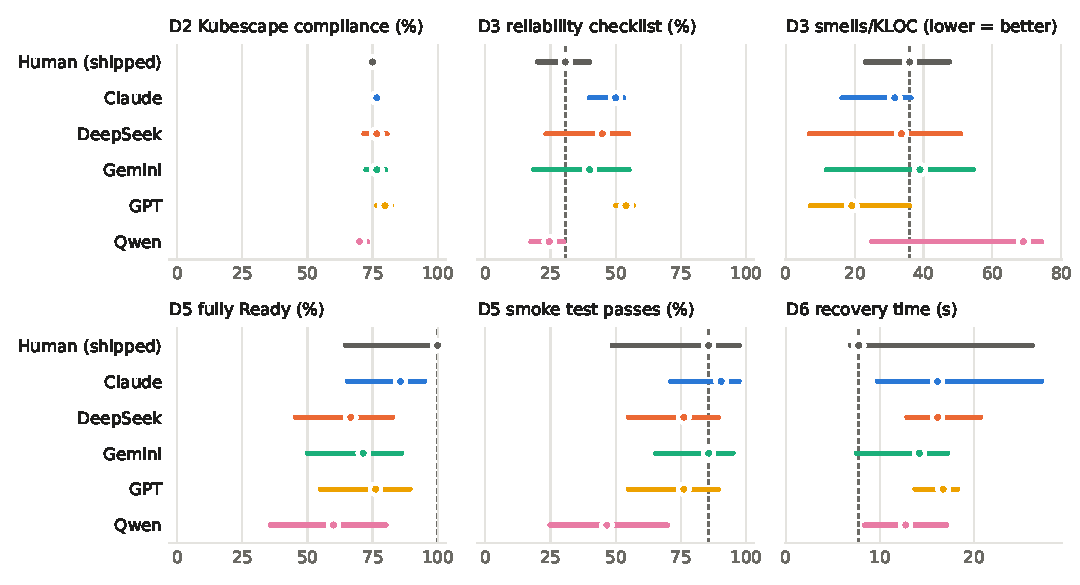
\includegraphics[width=\textwidth]{figures/fig_dimensions_neutral.pdf}
\caption{Neutral-prompt results per source. Dots show medians (continuous metrics) or proportions (binary metrics). Bars show interquartile ranges or 95\% Wilson intervals. The dashed line marks the human manifests. D1 and D4 are omitted because every source's median is 96--100\%. Human: $n=7$; Claude, DeepSeek, Gemini, GPT: $n=21$; Qwen: $n=15$; D6 is conditional on deployment.}
\label{fig:dimensions-neutral}
\end{figure*}

\textbf{Correctness (D1).} The API server accepted every object of every human manifest and of every neutral-prompt configuration from Claude, DeepSeek and GPT. Two of Gemini's 21 configurations, both for the Kubernetes Dashboard, are missing, because the provider withheld them for reproducing training data too closely. Qwen had every object accepted in only 10 of its 15 configurations. It mostly declared Services with several unnamed ports, which a schema validator accepts but the API server rejects.

\textbf{Security (D2).} The static security of the generated configurations is close to that of the shipped manifests. Median Kubescape compliance is 75.0\% for the human manifests, 76.7\% for Claude, DeepSeek and Gemini, 79.8\% for GPT and 70.0\% for Qwen. For every model, the project-level difference from the human manifests is within about ten points. This excludes large differences but not moderate ones. Few configurations reach the \texttt{restricted} Pod Security Standard (none of the human manifests; 0--24\% per model), while 84--100\% of every source passes \texttt{baseline}. The secret check flags 43\% of the human manifests and 52--64\% of each model's configurations, with no significant difference.

\textbf{Static reliability (D3).} Claude and GPT cover more of the reliability checklist than the shipped manifests (medians 50.0\% and 54.0\% against 30.7\%). This difference also holds at project level. Gemini (40.0\%), DeepSeek (44.9\%) and Qwen (24.5\%) are close to the human level.

\textbf{Requirements (D4).} Requirement satisfaction is high for every source (medians 96--100\%).

\textbf{Deployment (D5) and recovery (D6).} The models' configurations became fully Ready in 60\% (Qwen) to 86\% (Claude) of cases, and passed the smoke test in 47\% (Qwen) to 90\% (Claude). All seven human manifests became fully Ready, and six passed their smoke test. The exception, Sock Shop, became Ready, but its cart service failed: an image tag that the manifest leaves unpinned now resolves to an incompatible database release. We selected projects only if their human manifest could be deployed (Section~\ref{sec:method-dataset}). So the human rates are a reference, not a test. Every configuration that reached fault injection recovered from every fault, except one GPT configuration. Recovery took 7.8~s (median) for the human manifests and 13--17~s per model, a difference that is not significant.

In short, under the neutral prompt the models match the shipped manifests on static security, GPT and Claude cover more of the reliability checklist, and Qwen is lower on every static score.

\subsection{RQ2: Most frequent misconfigurations}\label{sec:res-rq2}

Table~\ref{tab:rahman} reports, for each source and prompt, the share of configurations showing each security misconfiguration category of \citet{rahman2023k8smisconfig}.

% generated by evaluation/tables.py -- do not edit
\begin{table*}[t]
\centering\small
\caption{Share of configurations (\%) exhibiting each security misconfiguration category of Rahman et al., detected with the rules of their SLI-KUBE tool. N = neutral prompt, P = production prompt. No configuration from any source exhibits activation of hostIPC, activation of hostNetwork, activation of hostPID, capability misuse, escalated privileges for child processes, privileged securityContext. Following SLI-KUBE, a hard-coded secret is any literal value under a key naming a user, password, token or secret. The D2 secret check of Table~\ref{tab:overview-neutral} is stricter (user names and placeholder values such as \texttt{changeme} are not counted, known credential token formats are), so its rates are lower.}\label{tab:rahman}
\resizebox{\textwidth}{!}{%
\begin{tabular}{lrrrrrrrrrrr}
\toprule
Category & Human & Claude N & Claude P & DeepSeek N & DeepSeek P & Gemini N & Gemini P & GPT N & GPT P & Qwen N & Qwen P \\ \midrule
Absent resource limit & 100 & 57 & 0 & 48 & 10 & 47 & 16 & 24 & 5 & 79 & 33 \\
Absent securityContext & 71 & 76 & 0 & 76 & 25 & 79 & 63 & 76 & 14 & 86 & 75 \\
Docker socket mounting & 0 & 14 & 0 & 14 & 5 & 16 & 16 & 10 & 0 & 7 & 0 \\
Hard-coded secret & 57 & 67 & 67 & 67 & 70 & 68 & 68 & 71 & 71 & 64 & 67 \\
Insecure HTTP & 0 & 14 & 14 & 14 & 10 & 16 & 16 & 14 & 14 & 21 & 25 \\
\bottomrule
\end{tabular}}
\end{table*}

Three categories dominate for every source:
\begin{itemize}
\item A hard-coded secret, by the SLI-KUBE rule, appears in 57\% of the human manifests and 64--71\% of each model's configurations under both prompts. The production prompt does not reduce it.
\item An absent security context appears in 71\% of the human manifests and 76--86\% of neutral-prompt configurations.
\item An absent resource limit appears in every human manifest and 24--79\% of neutral-prompt configurations.
\end{itemize}
For Claude, DeepSeek and GPT, the production prompt removes most of the last two (for Claude, from 57\% and 76\% to 0\%). Gemini and Qwen keep an absent security context in most configurations (63\% and 75\%). Docker socket mounting (7--16\% of neutral configurations) occurs only for Sock Shop: its Compose file mounts the socket, while its human manifest does not (Section~\ref{sec:disc-compose}).

Reliability settings are missing in a similar way (Appendix~\ref{app:stats}, Table~\ref{tab:checklist-items}). Under the neutral prompt, nearly every workload of every source, human manifests included, runs a single replica without a PodDisruptionBudget, anti-affinity or an explicit rolling-update strategy, and 35--68\% lack readiness and liveness probes. The production prompt adds these settings mainly for Claude and GPT (for Claude, single-replica workloads fall from 98\% to 23\%), partly for DeepSeek, and hardly at all for Gemini and Qwen.

\subsection{RQ3: Differences between models and consistency}\label{sec:res-rq3}

The models differ clearly in their static scores. GPT and Claude score highest, and Qwen and Gemini lowest, on Kubescape compliance, checklist coverage and Polaris score. Under the production prompt, the gap is larger: Claude, GPT and DeepSeek score higher than Gemini and Qwen on all three. Deployment success, however, does not differ significantly between models once the differences between projects are taken into account. These are comparisons of model-and-access configurations (Section~\ref{sec:method-generation}), not of models in isolation.

Gemini is the most consistent model: its three samples of a project usually receive the same Kubescape compliance and checklist coverage. Qwen is the least consistent. Whether a configuration works is less repeatable than its static scores. The three samples agree on becoming fully Ready in 86\% of cells for Claude, 71\% for Gemini, 50\% for GPT and Qwen and 43\% for DeepSeek, and on the smoke-test outcome in 64--71\% of cells for every model.

\subsection{RQ4: Why configurations fail at runtime, and whether static analysis predicts it}\label{sec:res-rq4}

Figure~\ref{fig:attrition} follows every configuration through the pipeline. Of the 198 generated configurations, 184 were schema-valid and 180 had every object accepted. But only 128 became fully Ready, 136 passed their smoke test and 118 did both. Most of the loss happens at deployment, not at validation, and it is larger under the production prompt.

\begin{figure*}[t]
\centering
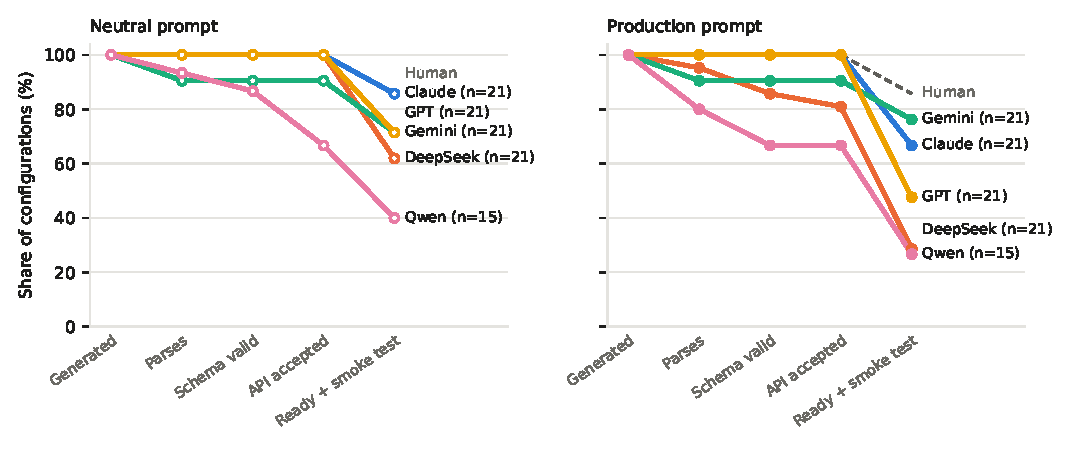
\includegraphics[width=\textwidth]{figures/fig_attrition.pdf}
\caption{Share of configurations surviving each stage, per model and prompt (open markers: neutral; filled: production). ``Ready + smoke'' is the share both fully Ready and passing the smoke test. Dashed line: the seven human manifests, which were selected for being deployable.}
\label{fig:attrition}
\end{figure*}

Being Ready and passing the smoke test are not the same. In 18 configurations, the application served every smoke-test request, but some workload never became Ready, most often an extra component copied from the Compose file, such as Sock Shop's load generator. In 10 others, every workload was Ready, but the application did not work, usually because a Service, RBAC object or NetworkPolicy on the request path was rejected or misdirected.

Table~\ref{tab:root-causes} gives the root cause of each of the 81 configurations (80 generated, one human) that were not both fully Ready and passing the smoke test. For 51, the cause is visible in the cluster's record; 22 are inferred, 5 are supported by a matched contrast and 3 remain undetermined. The most frequent causes are:
\begin{itemize}
\item host-level Compose services that fail while the application works (10);
\item invalid YAML or objects that the API server rejects (8);
\item hardening that stops a database (8);
\item liveness probes that kill slow-starting services (6).
\end{itemize}
The hardening and probe causes are concentrated under the production prompt (23 of their 30 failures).

% generated by evaluation/tables.py -- do not edit
\begin{table*}[t]
\centering\small
\caption{Root cause of every configuration that was not both fully Ready and passing its smoke test, by model and prompt (N = neutral, P = production). Obs.\ = cases whose mechanism is directly visible in the cluster's record (exit reason, log lines, events, rejected objects or provider stop reason); the remainder are inferred from the manifest together with the observed status, or, for two mechanisms, supported by a matched contrast.}\label{tab:root-causes}
\resizebox{\textwidth}{!}{%
\begin{tabular}{lrrrrrrrrr}
\toprule
Mechanism & Claude & DeepSeek & Gemini & GPT & Qwen & N & P & Human & Obs. \\ \midrule
\multicolumn{10}{l}{\textit{Hardening blocks the workload}} \\
\quad Capability drop or fixed UID stops the database & 3 & 3 & 0 & 2 & 0 & 0 & 8 & 0 & 3/8 \\
\quad runAsNonRoot on an image whose user cannot be verified & 0 & 1 & 0 & 2 & 0 & 1 & 2 & 0 & 0/3 \\
\quad Service-account token disabled for a component that needs the API & 0 & 0 & 0 & 1 & 0 & 0 & 1 & 0 & 1/1 \\
\quad NetworkPolicy blocks a documented internal route & 1 & 1 & 0 & 1 & 0 & 1 & 2 & 0 & 0/3 \\
\multicolumn{10}{l}{\textit{Probes and resource limits}} \\
\quad Liveness/startup probe kills a slow-starting service & 5 & 0 & 0 & 1 & 0 & 2 & 4 & 0 & 2/6 \\
\quad Memory limit too low (OOMKilled) & 0 & 1 & 0 & 1 & 0 & 1 & 1 & 0 & 2/2 \\
\quad Probe on the wrong port or path & 0 & 2 & 0 & 0 & 0 & 0 & 2 & 0 & 1/2 \\
\quad Probe calls a binary the image does not ship & 0 & 0 & 1 & 0 & 0 & 1 & 0 & 0 & 0/1 \\
\quad HTTP probe on a component without a server & 0 & 0 & 0 & 0 & 4 & 1 & 3 & 0 & 0/4 \\
\multicolumn{10}{l}{\textit{Compose file translated literally}} \\
\quad Host-level Compose services fail; application works & 1 & 2 & 6 & 1 & 0 & 7 & 3 & 0 & 10/10 \\
\multicolumn{10}{l}{\textit{Wrong values or references}} \\
\quad Service targets the wrong container port & 0 & 1 & 0 & 0 & 1 & 2 & 0 & 0 & 1/2 \\
\quad API server address overridden & 0 & 1 & 0 & 0 & 0 & 0 & 1 & 0 & 0/1 \\
\quad Volume references an undefined Secret & 0 & 1 & 0 & 0 & 0 & 1 & 0 & 0 & 1/1 \\
\quad RBAC does not allow updating the CSRF Secret & 0 & 0 & 0 & 1 & 3 & 2 & 2 & 0 & 0/4 \\
\quad No writable /tmp volume on a distroless image & 0 & 0 & 0 & 0 & 1 & 1 & 0 & 0 & 1/1 \\
\quad Image from a non-existent repository & 0 & 0 & 0 & 0 & 2 & 0 & 2 & 0 & 2/2 \\
\quad Required variable set to an empty value & 0 & 2 & 0 & 1 & 0 & 1 & 2 & 0 & 3/3 \\
\quad Non-existent command-line flag & 0 & 0 & 0 & 3 & 0 & 1 & 2 & 0 & 3/3 \\
\quad Placeholder domain enforced & 0 & 0 & 0 & 1 & 0 & 0 & 1 & 0 & 1/1 \\
\quad Points at a database host that does not exist & 0 & 1 & 0 & 1 & 0 & 1 & 1 & 0 & 2/2 \\
\quad TLS required by the client, not offered by the database & 0 & 1 & 0 & 0 & 0 & 0 & 1 & 0 & 1/1 \\
\multicolumn{10}{l}{\textit{Invalid or missing output}} \\
\quad Invalid YAML or object rejected by the API server & 0 & 1 & 0 & 0 & 7 & 4 & 4 & 0 & 8/8 \\
\quad RBAC object rejected (unquoted resource name) & 0 & 2 & 0 & 0 & 0 & 0 & 2 & 0 & 2/2 \\
\quad Reply ends before the YAML block closes & 0 & 0 & 1 & 0 & 2 & 1 & 2 & 0 & 3/3 \\
\quad Provider withheld the reply (recitation) & 0 & 0 & 3 & 0 & 0 & 2 & 1 & 0 & 3/3 \\
\multicolumn{10}{l}{\textit{Other}} \\
\quad Cause not determined & 0 & 2 & 0 & 1 & 0 & 2 & 1 & 0 & 0/3 \\
\quad Unpinned image tag drifted & 0 & 0 & 0 & 0 & 0 & 0 & 0 & 1 & 1/1 \\
\midrule
Total & 10 & 22 & 11 & 17 & 20 & 32 & 48 & 1 & 51/81 \\
\bottomrule
\end{tabular}}
\end{table*}

Higher static security and reliability scores show no positive association with deployment success (Figure~\ref{fig:static-runtime}). Configurations with higher scanner scores did not work more often, and this remains true when the prompt, the project and the model are taken into account (Appendix~\ref{app:stats}). Only requirement satisfaction is associated with success, and partly by construction: D4 checks that the documented components and settings are present, and without them a deployment cannot work.

\begin{figure*}[t]
\centering
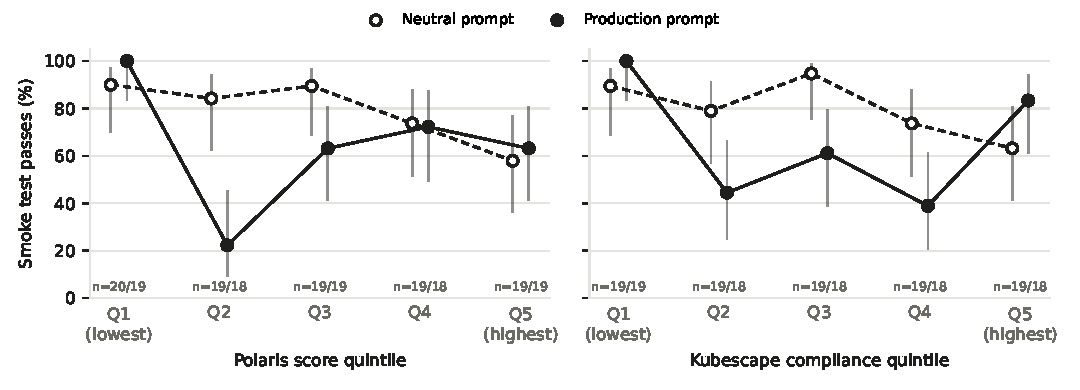
\includegraphics[width=\textwidth]{figures/fig_static_runtime.pdf}
\caption{Smoke-test pass rate by quintile of Polaris score (left) and Kubescape compliance (right), per prompt, with 95\% Wilson intervals. Neither score separates configurations that work from those that do not. $n$ = configurations per quintile (neutral/production); the adjusted analysis is in Appendix~\ref{app:stats}.}
\label{fig:static-runtime}
\end{figure*}

\subsection{RQ5: Effect of requesting production-ready output}\label{sec:res-rq5}

Figure~\ref{fig:tradeoff} summarises the effect for each model. Table~\ref{tab:overview-production} gives the production-prompt values.

% generated by evaluation/tables.py -- do not edit
\begin{table*}[t]
\centering\small
\caption{Six-dimension results, production prompt. Binary rows: percentage (count/n); continuous rows: median [interquartile range]. The human column is the shipped manifest of each project (one per project). Continuous rows are computed over the configurations for which the metric is defined: static scores over parsed configurations, D5 time to Ready and D6 over deployed ones, so their n can be smaller than the column total. D6 downtime depends mainly on the replica count of the faulted workload (Section~\ref{sec:res-rq5}).}\label{tab:overview-production}
\begin{tabular}{lrrrrrr}
\toprule
Metric & Human & Claude & DeepSeek & Gemini & GPT & Qwen \\ \midrule
Configurations & 7 & 21 & 21 & 21 & 21 & 15 \\ \midrule
D1 all objects API-accepted & 100 (7/7) & 100 (21/21) & 81 (17/21) & 90 (19/21) & 100 (21/21) & 67 (10/15) \\
D2 passes PSS baseline & 100 (7/7) & 100 (21/21) & 95 (19/20) & 84 (16/19) & 100 (21/21) & 100 (12/12) \\
D2 passes PSS restricted & 0 (0/7) & 62 (13/21) & 40 (8/20) & 16 (3/19) & 57 (12/21) & 0 (0/12) \\
D2 secret check flags a credential & 43 (3/7) & 57 (12/21) & 55 (11/20) & 58 (11/19) & 57 (12/21) & 67 (8/12) \\
D5 fully Ready & 100 (7/7) & 71 (15/21) & 43 (9/21) & 76 (16/21) & 57 (12/21) & 27 (4/15) \\
D5 smoke test passes & 86 (6/7) & 67 (14/21) & 38 (8/21) & 90 (19/21) & 57 (12/21) & 47 (7/15) \\
\midrule
D2 Kubescape compliance (\%) & 75.0 & 96.4 & 87.3 & 76.7 & 92.5 & 76.7 \\[-2pt]
 & {\scriptsize[73.0, 76.6]} & {\scriptsize[91.7, 100.0]} & {\scriptsize[84.1, 92.9]} & {\scriptsize[76.7, 84.3]} & {\scriptsize[89.8, 96.7]} & {\scriptsize[75.0, 79.7]} \\ \addlinespace[3pt]
D2 Trivy high+critical findings & 9.0 & 0.0 & 3.5 & 12.0 & 0.0 & 10.0 \\[-2pt]
 & {\scriptsize[1.0, 13.5]} & {\scriptsize[0.0, 4.0]} & {\scriptsize[1.0, 8.0]} & {\scriptsize[1.0, 15.0]} & {\scriptsize[0.0, 5.0]} & {\scriptsize[5.0, 12.8]} \\ \addlinespace[3pt]
D3 Polaris score & 62.0 & 90.0 & 85.0 & 71.0 & 86.0 & 69.5 \\[-2pt]
 & {\scriptsize[58.5, 72.5]} & {\scriptsize[86.0, 91.0]} & {\scriptsize[81.0, 87.5]} & {\scriptsize[68.0, 82.5]} & {\scriptsize[84.0, 89.0]} & {\scriptsize[65.2, 75.0]} \\ \addlinespace[3pt]
D3 reliability checklist (\%) & 30.7 & 80.7 & 64.0 & 55.2 & 75.0 & 41.2 \\[-2pt]
 & {\scriptsize[20.0, 40.0]} & {\scriptsize[70.0, 85.0]} & {\scriptsize[58.9, 79.2]} & {\scriptsize[52.5, 60.0]} & {\scriptsize[69.0, 79.0]} & {\scriptsize[30.0, 54.2]} \\ \addlinespace[3pt]
D3 smells per KLOC & 36.0 & 8.1 & 10.7 & 27.4 & 7.1 & 26.6 \\[-2pt]
 & {\scriptsize[23.1, 47.5]} & {\scriptsize[3.5, 10.4]} & {\scriptsize[1.7, 17.5]} & {\scriptsize[5.8, 43.2]} & {\scriptsize[0.0, 11.0]} & {\scriptsize[10.7, 42.7]} \\ \addlinespace[3pt]
D4 requirements met (\%) & 100.0 & 100.0 & 100.0 & 92.3 & 96.3 & 98.2 \\[-2pt]
 & {\scriptsize[95.8, 100.0]} & {\scriptsize[91.7, 100.0]} & {\scriptsize[93.7, 100.0]} & {\scriptsize[88.7, 98.2]} & {\scriptsize[91.7, 100.0]} & {\scriptsize[92.3, 100.0]} \\ \addlinespace[3pt]
D5 time to Ready (s) & 20.1 & 33.0 & 27.5 & 18.2 & 24.9 & 23.0 \\[-2pt]
 & {\scriptsize[14.6, 64.0]} & {\scriptsize[22.5, 42.8]} & {\scriptsize[16.6, 39.8]} & {\scriptsize[14.3, 35.0]} & {\scriptsize[18.6, 46.5]} & {\scriptsize[15.8, 32.5]} \\ \addlinespace[3pt]
D6 recovery time (s) & 7.8 & 15.0 & 14.6 & 13.7 & 9.2 & 17.1 \\[-2pt]
 & {\scriptsize[6.9, 26.2]} & {\scriptsize[10.9, 21.4]} & {\scriptsize[12.4, 22.7]} & {\scriptsize[8.5, 17.4]} & {\scriptsize[5.9, 17.9]} & {\scriptsize[15.6, 22.8]} \\ \addlinespace[3pt]
D6 downtime per fault (s) & 6.2 & 0.3 & 0.2 & 5.5 & 0.3 & 6.9 \\[-2pt]
 & {\scriptsize[2.8, 8.4]} & {\scriptsize[0.1, 6.0]} & {\scriptsize[0.2, 3.9]} & {\scriptsize[0.2, 7.0]} & {\scriptsize[0.2, 6.9]} & {\scriptsize[3.3, 8.4]} \\ \addlinespace[3pt]
\bottomrule
\end{tabular}
\end{table*}

\textbf{Static scores go up.} For the median model--project pair, the production prompt adds 9.1 points of Kubescape compliance, 22.5 points of checklist coverage and 13.3 points of Polaris score, and removes 3.5 high or critical Trivy findings and 16.9 smells per thousand lines. The gain is largest for Claude (Kubescape $+19.8$ points), then GPT ($+12.4$) and DeepSeek ($+10.1$), and small for Qwen ($+5.7$) and Gemini ($+3.6$). In addition, 27 configurations pass the \texttt{restricted} Pod Security Standard only under the production prompt, and one only under the neutral one.

\textbf{Deployment success goes down.} The smoke-test pass rate falls from 76.8\% (76 of 99) to 60.6\% (60 of 99), and the fully Ready rate from 72.7\% to 56.6\%. Across model--project pairs, the fully Ready rate falls in 13 and rises in 3, and the smoke-test rate falls in 12 and rises in 3; both declines are significant. Gemini is the exception: its rates are nearly the same under both prompts (Figure~\ref{fig:tradeoff}), and its scores also changed least. The added failures are those of Section~\ref{sec:res-rq4}: hardening that stops a database and liveness probes that kill slow-starting services.

% Full-width float: a one-column float queues behind the earlier full-width figure, and an inline one leaves gaps
\begin{figure*}[t]
\centering
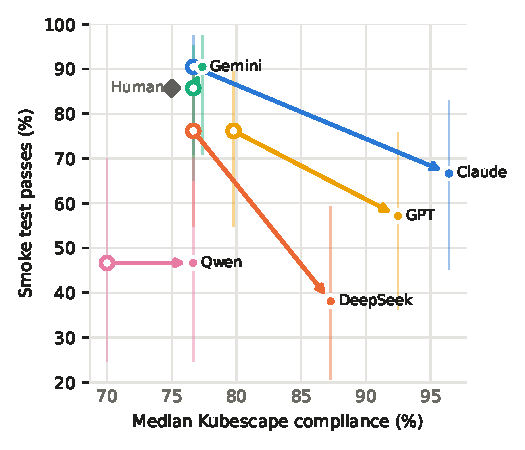
\includegraphics[width=0.55\textwidth]{figures/fig_tradeoff.pdf}
\caption{Static security against deployment success, per model. Open marker = neutral prompt, filled = production prompt (vertical bars: 95\% Wilson intervals of the smoke-test rate); diamond = human manifests. Two coincident markers (Claude neutral, Gemini production) are offset slightly.}
\label{fig:tradeoff}
\end{figure*}

\textbf{Recovery does not change.} Every configuration that recovered from all faults under one prompt also did under the other. Downtime during a fault depends almost entirely on the number of replicas: about 6--7~s with one replica, for every source, and 0.2~s with two or more. The production prompt gives the faulted workload two or more replicas in 55\% of configurations, against 12\% under the neutral prompt and none of the human manifests.
\section{Discussion}\label{sec:discussion}

% Counts are taken from evaluation/d5_root_causes.csv, evaluation/analysis/report.md and robust_report.md.

\subsection{Hardening that breaks the workload it hardens}\label{sec:disc-hardening}

Under the production prompt, one recurring cause of failure is a security control that ignores the image it constrains. Eight configurations hardened their database so that it could not start. Three each came from Claude and DeepSeek and two from GPT, all under the production prompt. In seven, the database container (PostgreSQL in six, MySQL in one) keeps its root-based entrypoint but has every Linux capability dropped. The entrypoint must take ownership of its data directory and then switch to an unprivileged user. Without the corresponding capabilities, it can do neither. In the eighth, the database runs as a fixed non-root user. Its data directory is at the root of a volume it does not own, so initialisation cannot set the directory's permissions. These eight configurations score as well on Kubescape as the other production-prompt configurations (median compliance 89.6\% in both groups). So the scanner gives no sign of the defect.

Two further mechanisms follow the same pattern. Each is a recognised practice in isolation. The first is a liveness or startup probe whose time budget is shorter than a slow-starting Java service needs. It kills each container before it finishes starting, so the services restart indefinitely. This accounts for six failures (five from Claude, four under the production prompt). We observed it directly in two: the kubelet killed them with no out-of-memory reason, and log lines showed the services still initialising. For the other four, we inferred it from the same probe settings and readiness record. The second is a least-privilege NetworkPolicy that admits traffic to the Kubernetes Dashboard's metrics scraper only from the dashboard's own pods. It blocks the dashboard's default route to the scraper, which passes through the API server's service proxy. Samples from the same model with an identical policy but a direct scraper address connected normally. This accounts for two failures. Neither rests on a controlled experiment: one is supported by that matched contrast, the other inferred from the same policy. The third NetworkPolicy failure in Table~\ref{tab:root-causes} has a different mechanism. An Online Boutique policy admits internal traffic only from pods with a label that no pod carries.

So the production prompt buys static compliance partly at the cost of deployability (Section~\ref{sec:res-rq5}). Static gains matter only for configurations that still deploy.

\subsection{Translating the Compose file too literally}\label{sec:disc-compose}

Every model receives the project's Docker Compose file, and models tend to translate it service by service. This faithfulness is a defect when the Compose file reflects a Docker-host setup that the maintainers deliberately left out of their Kubernetes manifests. Sock Shop's Compose file mounts the host's Docker socket into one service and runs a one-shot load generator. Its Kubernetes manifest contains neither. Under the neutral prompt, 12 of the 15 Sock Shop configurations mount the socket (all three samples from Claude, DeepSeek and Gemini). Under the production prompt, 4 of 15 do so. Also, 27 of the 30 include the load generator. Access to the Docker socket is equivalent to root on the node \citep{rahman2023k8smisconfig}. The socket also does not exist on nodes whose container runtime is not Docker Engine, as on the evaluation cluster. A load generator run as a long-lived Deployment restarts indefinitely. In several samples, its command also calls a start-up script that does not exist in the image. The load generator is the most frequent single cause of a configuration that serves correctly but is not fully Ready (Table~\ref{tab:root-causes}).

\subsection{What static analysis misses}\label{sec:disc-static}

Several failures were not visible to the static scanners. The cluster records a memory limit too tight for a Java service as an out-of-memory kill. But no scanner relates a limit to the workload it constrains. A database that cannot start under its security context passes every structural check. So does a probe aimed at a path the image does not serve. Other defects are caught before deployment but are easy to miss in review. In two DeepSeek configurations, YAML parsed an unquoted RBAC resource name containing colons as a mapping. The API server then rejected the whole Role, and the dashboard started without its permissions. Consistent with these cases, higher static security and reliability scores show no positive association with deployment success (Section~\ref{sec:res-rq4}). Only requirement satisfaction, which checks that the documented components and settings are present, is weakly associated with it. Each of these defects surfaced only at deployment.

\subsection{``Ready'' is not the same as ``working''}\label{sec:disc-ready}

Kubernetes considers a workload Ready when its readiness probe passes, or immediately if it has none. The human Sock Shop manifest defines no readiness probes. So its slow Java services are reported Ready long before they accept connections. Yet several generated configurations serve every request correctly while an auxiliary workload is not Ready. In this study, the two outcomes disagree for 28 of the 198 generated configurations. Of these, 18 serve correctly without being fully Ready, and 10 are fully Ready without serving correctly. Reporting both readiness and a smoke test avoids rewarding missing probes and penalising non-essential components.

\subsection{Memorisation}\label{sec:disc-memorisation}

Two observations relate to the contamination threat (Section~\ref{sec:threats}). First, Gemini's provider withheld three responses for the Kubernetes Dashboard (two under the neutral prompt, one under the production prompt). The reason was that they reproduced training data too closely. The project's official manifest is widely published. Second, some models' configurations are more similar to the published human manifest than to the other models' configurations for the same project. This pattern is expected if a published manifest is being reproduced. The excess is clearly positive for Claude on the Kubernetes Dashboard (Jaccard $+0.35$) and Emojivoto ($+0.23$) and for Gemini on Sock Shop ($+0.23$). It is close to zero or negative elsewhere. For Claude, the session transcripts rule out access to the human manifests during generation (Section~\ref{sec:method-generation}). So this similarity reflects what the model learned in training. Neither observation affects the scoring. But both limit how far results on widely published projects can be read as reasoning from documentation.

\subsection{Generalisation beyond the evaluated projects}\label{sec:disc-generalisation}

The failure mechanisms above come from how generated configurations interact with common images and Kubernetes defaults, not from any single application. Database images with root-based entrypoints, slow-starting JVM services and Compose files written for a Docker host are widespread. So we expect these mechanisms to recur in similar projects. This expectation remains to be tested. The per-project rates reported here should not be extrapolated to applications of other kinds.

\subsection{Implications}\label{sec:disc-implications}

For practitioners, the results suggest three checks before adopting a generated configuration. First, deploy it and exercise it, rather than relying on how it reads or scores. Second, review every hardening setting against the documented behaviour of the image it constrains. In particular, check capability drops and fixed user IDs on database images, and liveness probes on slow-starting services. Third, treat host-level settings carried over from a Compose file (socket mounts, host paths, one-shot services) as suspect. Asking a model for ``production-ready'' output makes these checks more necessary, not less. For tool builders, the results suggest scanner rules that relate a security setting to the image it is applied to. For researchers, benchmarks of generated infrastructure code should include execution, because a scanner score did not indicate which configurations would work.
\section{Threats to Validity}\label{sec:threats}

\textbf{Model access.} The models were reached through different routes (Table~\ref{tab:models}). This is a known risk for studies that use LLMs \citep{sallou2024breaking}. Three were used through conversational interfaces rather than a raw API. Claude ran through Claude Code subagents, whose harness adds its own system prompt to ours. GPT and DeepSeek ran through their web chats, whose own system prompts and defaults are outside the study's control. So temperature and the output limit were controlled only for Gemini and Qwen. This affects the consistency comparison of RQ3 more than any other result. GPT was generated with ChatGPT's default model, so its exact version is not known. It answered with a medium reasoning effort, left unchanged. One author (T.~Hussain) operated its web sessions following a written protocol: a new temporary, unpersonalised chat per prompt, no tools, no follow-up, and replies copied unedited. Adherence to this protocol was not independently observed. For 16 of its 42 prompts, the interface turned the pasted prompt into an attached file with identical content. They came from the three projects with the longest documentation. Gemini is a flash-tier model rather than the planned Pro tier. Its hidden reasoning tokens count against its 8,192-token output limit. Qwen's free tier rejects the prompts of the two largest projects, so its missing cells reflect access, not quality. A sixth model, Llama, was dropped before the main run because no working access route was found.

\textbf{Training-data contamination.} All projects are public, and only two of the seven manifest repositories have fewer than 2,000 GitHub stars. So a model may reproduce a memorised manifest rather than reason from the documentation. We record provider refusals for recitation. We also compare each model's similarity to the human manifest with its similarity to the other models' configurations for the same project. Only an excess over this peer level is read as reproduction (Section~\ref{sec:disc-memorisation}). Reproduction would pull a model's configurations toward the human manifest, and so shrink the differences reported for RQ1.

\textbf{Selection of projects and of the human baseline.} Results describe these seven projects, not application classes in general (Section~\ref{sec:disc-generalisation}). The set was fixed after a two-project pilot and before the main run. A project was selected only if its human manifest deployed on the evaluation cluster. So the human D5 outcomes are partly true by construction, and the selection favours applications that run on a local cluster. Human runtime results are therefore reported as a reference only.

\textbf{Evaluation cluster.} D5 and D6 are measured on a four-node \texttt{kind} cluster on a single host. Cloud load balancers, multi-zone scheduling and production storage are not exercised. Absolute times should not be read as representative of production. \texttt{kind}'s local-path storage does not apply a pod's \texttt{fsGroup}, which could make a database fail here that would start elsewhere. None of the eight database failures depends on it. Seven run the container as root with every capability dropped, which prevents the entrypoint from changing file ownership or switching user, whatever the volume's group. The eighth fails because another user owns its data directory, and \texttt{fsGroup} does not change that.

\textbf{Measurement adjustments.} The pipeline was corrected 25 times during the study (Appendix~\ref{app:fixes}). Each correction was logged with its trigger, applied to every configuration it could affect, and followed by re-evaluation. All were made after generation had begun. Most were found while diagnosing failures, so they are one-sided. Of the corrections, 8 affected only the running of the pipeline and 3 made scoring stricter. The other 14 removed a failure that the investigation traced to the measurement or to an undocumented prerequisite. They never removed a success that turned out to be spurious. Appendix~\ref{app:fixes} separates corrections of the measurement from changes to an outcome's definition and from supplied prerequisites. Among the definition changes that removed failures, Correction~19 leaves a strict variant of D6, which is reported alongside. Correction~26 changes the outcome of two configurations (DeepSeek, Grafana, production prompt). Without it, the production smoke-test rate would be 58 rather than 60 of 99. Two corrections (2 and 10) were triggered by failures of human manifests. The deployment results are robust to leaving out any one project (Section~\ref{sec:res-rq5}). Two adjustments supply facts that the bundles lack (image aliases and start-up prerequisites, Section~\ref{sec:method-pipeline}). They apply to 29 generated configurations and to no human manifest. Take the worst case, in which every adjusted configuration that succeeded would otherwise have failed. Then the share of generated configurations both fully Ready and passing the smoke test falls from 59.6\% to 51.0\%. Four of the dashboard failures concern a start-up Secret that the documentation never mentions. Once the Secret is supplied, these configurations fail because their RBAC rules do not let the dashboard update it. A deployer would also have to discover this. Three configurations set a required variable to an empty string, which the application rejects. The start-up adjustment fires only when a variable is absent, so they are scored as failing.

\textbf{Labelling and tools.} Root-cause labels were assigned by a single rater. They were drafted with the help of an AI assistant from the same model family as one of the evaluated models (Claude). The blind second labelling pass was also made by a Claude model, not by a second human. It shows that the labels follow from the recorded evidence ($\kappa=0.84$). But it cannot rule out errors that models of one family share. The evidence level of each label is reported. Every label is published with its evidence so that it can be re-rated. The static tools are imperfect and disagree with one another. So we read their findings as what these pinned tool versions detect. We report the agreement between the two security scanners. Redaction decisions followed a written rule set. Every redaction was logged and reviewed by a second author, but borderline cases remain possible. Facts that the bundles do not contain are excluded from D4. However, the default ports of widely used database images are treated as general knowledge and scored.

\textbf{Resilience measurement.} Kubernetes controllers handle the two injected faults whatever the configuration says. So recovery success barely discriminates, and downtime depends mainly on replica count. D6 therefore characterises the replica choices a model makes, not a broader notion of resilience. Faults such as node drains or resource pressure would test more of a configuration's choices.

\textbf{Drift.} Providers update the weights behind a model identifier without notice. An unpinned image tag resolves to whatever is current. Generation dates are recorded for every configuration, and images were resolved in November 2026. Tag drift affects the human baselines too. The human Sock Shop manifest references \texttt{mongo} without a tag. It now resolves to a release whose wire protocol the project's 2017 cart service no longer speaks. Re-deploying with the image pinned to an older release passed, but the baseline is scored as published.
\section{Conclusion}\label{sec:conclusion}

This study compared Kubernetes configurations generated by five current LLMs with the manifests shipped by the same seven open-source projects. Every configuration was deployed and exercised, not only scanned. Each model received only the project's own documentation, under a neutral and a production-oriented prompt, three times each.

First, generated configurations are largely valid: 92.9\% are schema-valid, and requirement satisfaction is high for every model. Under a neutral prompt, their static security is close to what these projects ship (within about ten Kubescape points per model). GPT's and Claude's also cover more of the reliability checklist. But validity does not imply a working deployment. Only 59.6\% of the generated configurations became fully Ready and passed their smoke test. Higher static security and reliability scores showed no positive association with success. Second, asking for production-ready output raises static scores but lowers deployment success. Across model--project cells, median Kubescape compliance rose by 9 points and checklist coverage by 22.5. Yet the smoke-test pass rate fell from 76.8\% to 60.6\%. The added failures come from hardening applied without regard to the image (capability drops that stop databases from starting, liveness probes that kill slow-starting services). Third, models translate a project's Docker Compose file too literally. They carry over host-level settings, such as a mounted Docker socket, that the maintainers deliberately left out of their Kubernetes manifests.

A generated configuration should therefore be deployed and exercised before it is trusted. Its hardening settings should be checked against the images they constrain. Future work should extend the evaluation to more projects, to managed multi-node clusters and to faults that exercise configuration choices (node drains that test disruption budgets, resource pressure, dependency restarts). It should also test whether the cluster's record of a failed deployment lets a model repair its own configuration. Here, this record identified a cause for nearly every failure.

\FloatBarrier
\appendix
\section{Measurement instruments and pipeline corrections}\label{app:fixes}

\begin{table}[t]
\centering\small
\caption{Outcome instruments per project. D4: scored and oracle checks. Smoke test: steps in order. Each step is an HTTP request with an expected status and content, except the data-store checks, which run a command in the data-store container. Only Correction~26 (Appendix~\ref{app:fixes}) changed a check's criterion after results were seen. Corrections 5, 17, 20, 21 and 25 changed where the client runs, not what it checks.}\label{tab:instruments}
\resizebox{\columnwidth}{!}{%
\begin{tabular}{lrp{0.62\columnwidth}}
\toprule
Project & D4 & Smoke-test steps \\ \midrule
n8n & 13/0 & health endpoint; readiness including the database; n8n schema present in PostgreSQL \\
Grafana & 3/0 & API health reports the database as ok; login page; data store present (SQLite file, or PostgreSQL or MySQL as documented) \\
Voting app & 12/0 & vote page; result page; cast a vote; vote stored in the database \\
Emojivoto & 12/0 & web page; emoji list; cast a vote; leaderboard shows the vote \\
Online Boutique & 11/43 & home page lists products; product page; add to cart; view cart; cart stored in Redis; checkout completes \\
Sock Shop & 27/7 & home page; catalogue; tags; demo-user login; cart read \\
Dashboard & 7/11 & UI page; API-server health; metrics-scraper health; dashboard reaches the scraper \\
\bottomrule
\end{tabular}}
\end{table}


Table~\ref{tab:fixes} lists every correction to the evaluation pipeline, in the order made (the log numbers them 2--27; no corrections 1 and 18 were recorded). Of the 25, 8 are B, 9 are M, 5 are D and 3 are P (definitions in the caption). Effect: $+$ removes a failure that the investigation traced to the measurement or to an undocumented prerequisite; $-$ makes scoring stricter; 0 affects only the running of the pipeline. Each correction was applied to every configuration it could affect, followed by re-evaluation.

\begin{table*}[t]
\centering\footnotesize
\caption{Pipeline corrections (kind, trigger, change and effect). Kind: B = bug in running or recording the pipeline; M = the measurement itself was wrong; D = an outcome's definition changed; P = a prerequisite the documentation omits is supplied. $^{H}$ = first observed on a human manifest. All dates are November 2026.}\label{tab:fixes}
\begin{tabular}{rllp{0.34\textwidth}p{0.34\textwidth}c}
\toprule
\# & Kind & Date & Trigger & Change & Effect \\ \midrule
2 & M$^{H}$ & 8 & Human Online Boutique services killed by probes while images were still pulling & Images pre-pulled before deployment & $+$ \\
3 & P & 9 & Every Online Boutique front end exits: variable required only in source code & Variable supplied when absent & $+$ \\
4 & B & 9 & Hung namespace deletion discarded a finished result & Cleanup timeout is a warning & 0 \\
5 & M & 9 & Smoke client blocked by a configuration's own NetworkPolicy & Client placed where policies admit it & $+$ \\
6 & P & 9 & Two Online Boutique services exit unless a cloud profiler is disabled & Variable supplied when absent & $+$ \\
7 & D & 9 & Crash-looping pods counted Ready at an instant & Ready requires 20 s without interruption & $-$ \\
8 & B & 9 & API errors recorded as empty pod lists & Retry, then abort without a record & 0 \\
9 & B & 9 & API key written to a log & Key sent in a header; log redacted & 0 \\
10 & M$^{H}$ & 9 & Human Sock Shop database exhausted host memory & Open-files limit set to Docker's default & $+$ \\
11 & B & 11 & Empty Gemini reply crashed the generator & Empty reply recorded as output & 0 \\
12 & M & 11 & StatefulSet pod replacement never detected in D6 & Pods matched by UID, not name & $+$ \\
13 & B & 11 & Batch driver skipped models & Loop variable fixed & 0 \\
14 & D & 11 & Duplicate YAML keys silently merged & Duplicate keys rejected, as by \texttt{kubectl} & $-$ \\
15 & B & 11 & Empty Kubescape output crashed the evaluation & Treated as a scanner failure & 0 \\
16 & D & 11 & Empty reply counted as parsed & At least one document required & $-$ \\
17 & M & 11 & Client placement ignored named ports & Named ports resolved & $+$ \\
19 & D & 11 & Auxiliary workload blocked D6 although the application served & D6 runs if Ready or smoke-test passes; strict variant reported & $+$ \\
20 & M & 12 & One client used for checks needing different network access & Client placed per check & $+$ \\
21 & M & 12 & Client rejected by a namespace enforcing the restricted standard & Client complies with it & $+$ \\
22 & B & 12 & Schema downloads timed out & Schemas cached & 0 \\
23 & M & 12 & Transient pull failure could be scored as unpullable & Only definitive failures count & $+$ \\
24 & B & 12 & Stopped cluster passed the health check & Health check queries the control plane & 0 \\
25 & M & 14 & Client refused by a configuration's resource quota & Client declares requests and limits & $+$ \\
26 & D & 14 & Data check required Grafana's embedded database & PostgreSQL and MySQL also accepted, as documented & $+$ \\
27 & P & 14 & Dashboard exits without a Secret named only in source code & Empty Secret supplied when absent & $+$ \\
\bottomrule
\end{tabular}
\end{table*}

\section{Statistical details}\label{app:stats}

% Numbers come from evaluation/analysis/report.md (stats.py) and evaluation/analysis/robust_report.md (robust.py).
This appendix gives the statistical tests behind the statements in Section~\ref{sec:results}.

\subsection{Analysis approach}

Configurations are clustered. The three samples of a (model, project, prompt) cell share their input, and the projects differ widely. So, wherever the question allows, inference treats the project or the (model, project) cell as the unit. Configuration-level tests are reported as descriptive support. Binary outcomes are shown with 95\% Wilson intervals \citep{wilson1927probable}.

\emph{RQ1} compares each model's neutral-prompt configurations with the human manifests at configuration level. For continuous metrics, it uses the Kruskal--Wallis test \citep{kruskal1952ranks} followed by Dunn's test \citep{dunn1964multiple}. For binary ones, it uses Fisher's exact test. The effect size is Cliff's $\delta$ \citep{cliff1993dominance} (negligible $<0.147$, small $<0.33$, medium $<0.474$, large otherwise \citep{romano2006appropriate}). Only seven human configurations exist, so we repeat RQ1 at project level. Each model's mean over the three samples of a project is paired with that project's human manifest. With $n\le7$ pairs, a Wilcoxon test adjusted over five models cannot reach $p<0.078$. So this analysis reports Hodges--Lehmann differences with exact 95\% intervals. \emph{RQ3} compares the five models with a Friedman test \citep{friedman1937ranks} blocked on project, over the five projects every model completed. The effect size is Kendall's $W$. Five blocks are too few for the $\chi^2$ approximation, so $p$-values come from 20,000 within-block permutations. Configuration-level Kruskal--Wallis tests are reported alongside. Consistency is the across-sample standard deviation of each metric within a cell and the share of cells whose three samples agree on the runtime outcome. \emph{RQ5} pairs the two prompts at the (model, project) cell. It compares the cell's mean (or pass rate) under each prompt with the Wilcoxon signed-rank test. Pairing individual samples is not meaningful, because the sample index carries no information across prompts. As a secondary view, we report exact McNemar tests \citep{mcnemar1947note} on configuration pairs. We report per-model effects as Hodges--Lehmann estimates, and heterogeneity between models with a Kruskal--Wallis test on the per-cell changes. We check robustness by leaving out one project at a time. \emph{RQ4} models each binary runtime outcome with a logistic regression on one standardised static score. Prompt and project are fixed effects, and standard errors are clustered by (model, project) cell \citep{cameron2015cluster}. A second specification adds model fixed effects. A cluster bootstrap over cells (999 replicates) checks the sandwich intervals. RQ2 reports frequencies. We measure agreement between Kubescape and Trivy on their overlapping checks with Cohen's $\kappa$ \citep{cohen1960kappa}.

$P$-values are adjusted with the Holm procedure \citep{holm1979simple} within explicitly defined families: the pairwise comparisons after one omnibus test; the five per-model tests of one metric; the three static scores (and, separately, the two deployment outcomes) of one prompt in RQ3; the ten score--outcome models of each RQ4 specification; and, in RQ5, the six static measures and, separately, the two deployment outcomes. The other RQ5 comparisons (requirement satisfaction, time to Ready and the D6 measures) are secondary and reported unadjusted.

\subsection{RQ1}

\textbf{Correctness.} The share of accepted objects differs across sources (Kruskal--Wallis $H=21.81$, $p<0.001$) only because of Qwen (Dunn, $p\le0.049$ against the human manifests, Claude, DeepSeek and GPT).

\textbf{Security.} Kubescape compliance differs across sources ($H=24.50$, $p<0.001$). GPT (Cliff's $\delta=+0.565$, large) and Claude ($+0.327$, small) lie above the human manifests, and Qwen ($-0.637$, large) below them. However, none of these differences survives adjustment. The significant pairs are Claude--Qwen and GPT--Qwen. For the secret check, the omnibus test gives $\chi^2=1.08$, $p=0.956$, and every pairwise Fisher test against the human manifests gives $p=1.000$.

\textbf{Reliability and requirements.} For checklist coverage, Claude and GPT have $\delta=+0.50$ and $+0.72$, and the GPT--human difference is significant at configuration level ($p=0.040$). KubeLinter smell density does not differ significantly between sources ($H=9.62$, $p=0.087$), and neither does requirement satisfaction ($H=10.47$, $p=0.063$).

\textbf{Deployment and recovery.} No pairwise difference in deployment outcomes with the human manifests is significant (Fisher, all $p\ge0.60$). Time to Ready does not differ ($H=5.84$, $p=0.322$), and neither does recovery time ($H=1.77$, $p=0.880$).

\textbf{Project level.} Table~\ref{tab:rq1-hl} reports the project-level Hodges--Lehmann differences. The intervals for Kubescape compliance and Polaris score include zero for every model; the widest Kubescape interval is GPT's, $-5.3$ to $+9.9$. GPT's and Claude's checklist coverage is higher than the human manifests' ($+20.4$ points, 95\% CI $+5.6$ to $+37.5$, and $+11.1$, CI $+0.5$ to $+30.0$; unadjusted). Restricting the configuration-level comparison to the five projects every model completed leaves the pattern unchanged (for GPT, checklist $\delta=+0.93$). The two production-oriented human manifests (Grafana and the Kubernetes Dashboard) score below most models on Kubescape compliance and checklist coverage. Their large effect sizes cannot be tested meaningfully with only two human configurations.

\begin{table}[t]
\centering\small
\caption{RQ1 at project level: Hodges--Lehmann difference (model $-$ human) with exact 95\% CI, over the projects' mean neutral-prompt scores ($n=7$ projects; Qwen $n=5$). Rates in percentage points. A project's smoke-test rate takes values in thirds, so that column is coarse.}\label{tab:rq1-hl}
\resizebox{\columnwidth}{!}{%
\begin{tabular}{lrrr}
\toprule
Model & Kubescape (pts) & Checklist (pts) & Smoke test (pp) \\ \midrule
Claude & $+1.4$ [$-4.7$, $+4.4$] & $+11.1$ [$+0.5$, $+30.0$] & $0$ [$0$, $+17$] \\
DeepSeek & $-0.1$ [$-5.3$, $+5.6$] & $+6.9$ [$-10.7$, $+25.0$] & $0$ [$-50$, $+33$] \\
Gemini & $-0.1$ [$-4.9$, $+4.8$] & $+1.6$ [$-10.4$, $+20.0$] & $0$ [$-33$, $+50$] \\
GPT & $+5.9$ [$-5.3$, $+9.9$] & $+20.4$ [$+5.6$, $+37.5$] & $0$ [$-50$, $+33$] \\
Qwen & $-2.5$ [$-9.4$, $+0.3$] & $+6.2$ [$-7.8$, $+25.0$] & $-33$ [$-100$, $0$] \\
\bottomrule
\end{tabular}}
\end{table}

\subsection{RQ2}

Kubescape and Trivy largely agree on the five checks that both implement (Cohen's $\kappa=0.88$ overall, 0.70--1.00 per check). Table~\ref{tab:checklist-items} gives the share of workloads missing each reliability checklist item. Under the production prompt, missing PodDisruptionBudgets fall from 100\% to 34\% for Claude, and every workload from Claude, DeepSeek and GPT sets resource requests and limits.

% generated by evaluation/tables.py -- do not edit
\begin{table*}[t]
\centering\small
\caption{Share of applicable workloads (\%) missing each item of the Reliability Controls Checklist, pooled over all configurations of a source and prompt. N = neutral prompt, P = production prompt.}\label{tab:checklist-items}
\resizebox{\textwidth}{!}{%
\begin{tabular}{lrrrrrrrrrrr}
\toprule
Missing item & Human & Claude N & Claude P & DeepSeek N & DeepSeek P & Gemini N & Gemini P & GPT N & GPT P & Qwen N & Qwen P \\ \midrule
Two or more replicas & 100 & 98 & 23 & 92 & 54 & 99 & 76 & 93 & 31 & 97 & 93 \\
Readiness probe & 60 & 40 & 9 & 50 & 23 & 57 & 50 & 45 & 10 & 68 & 66 \\
Liveness probe & 55 & 35 & 9 & 48 & 26 & 56 & 50 & 45 & 10 & 68 & 63 \\
CPU request & 35 & 21 & 0 & 42 & 0 & 54 & 12 & 3 & 0 & 76 & 19 \\
Memory request & 43 & 21 & 0 & 42 & 0 & 54 & 12 & 3 & 0 & 76 & 19 \\
Memory limit & 45 & 21 & 0 & 42 & 0 & 54 & 12 & 3 & 0 & 76 & 18 \\
Explicit rolling update & 98 & 100 & 52 & 98 & 80 & 98 & 100 & 98 & 43 & 100 & 100 \\
PodDisruptionBudget & 100 & 100 & 34 & 100 & 76 & 100 & 100 & 99 & 48 & 100 & 100 \\
Anti-affinity or spread & 100 & 100 & 66 & 100 & 95 & 100 & 100 & 100 & 96 & 100 & 100 \\
Pinned image tag & 18 & 36 & 7 & 36 & 33 & 10 & 19 & 26 & 7 & 11 & 8 \\
\bottomrule
\end{tabular}}
\end{table*}

Measured the same way, the models' KubeLinter smell densities are comparable to the human manifests'. The exception is that 10.8--16.1 containers per thousand lines may run as root, against 7.7. They are lower than those \citet{zhang2024genaismells} reported for ChatGPT manifests of 2023. However, the units differ (whole multi-object configurations here, mostly single-object files there), so the comparison is not like for like.

\subsection{RQ3}

Blocked on project (Friedman test over the five common projects, permutation $p$-values Holm-adjusted over the three scores of each prompt), the models differ under the neutral prompt in Kubescape compliance ($\chi^2=10.63$, adjusted $p=0.019$, $W=0.53$), checklist coverage ($\chi^2=13.29$, $p=0.005$, $W=0.66$) and Polaris score ($\chi^2=13.60$, $p=0.005$, $W=0.68$). Under the production prompt, $\chi^2\ge16.48$, adjusted $p<0.001$ and $W\ge0.82$. Configuration-level tests over all projects agree ($H=60.80$, $46.91$ and $49.19$ for the production prompt). Requirement satisfaction differs between models only under the neutral prompt, and only between Gemini and GPT ($H=10.27$, $p=0.036$; Dunn $p=0.030$).

For deployment success, the adjusted permutation $p$ are $0.864$ (neutral) and $0.209$ (production) for becoming fully Ready, and $0.241$ and $0.209$ for the smoke test. At configuration level, the smoke-test rate does differ (neutral $\chi^2=10.78$, $p=0.029$; production $\chi^2=13.95$, $p=0.007$, Gemini 90\% against DeepSeek 38\%), but these differences do not persist once projects are blocked, although five blocks give this test little power.

The median across-sample standard deviation is 0 for Gemini on Kubescape compliance and checklist coverage. For Qwen it is 15.8 points for the share of objects accepted and 11.1 for checklist coverage. Gemini and Qwen, the two models whose temperature was fixed, lie at opposite ends, so access settings alone do not explain the differences.

\subsection{RQ4}

Pooled over both prompts, configurations with higher Polaris scores and Kubescape compliance pass the smoke test less often ($r_{pb}=-0.29$ and $-0.23$, Holm-adjusted $p<0.001$ and $p=0.026$), and those with more KubeLinter smells pass it more often ($+0.28$, $p=0.001$). Part of this reflects the prompt, which raises static scores and lowers success together. Table~\ref{tab:rq4} holds prompt and project fixed and clusters errors by cell. The odds ratios per standard deviation of the four scanner-based scores do not differ significantly from 1 for either outcome after adjustment. The point estimates for the smoke test are below 1 (Kubescape 0.46, Polaris 0.47), and lower still with model fixed effects (0.24 and 0.19), whose unadjusted intervals exclude 1 but whose adjusted $p$ are 0.082 and 0.165. So the data give no sign that higher scores go with working deployments, without establishing that they go with failing ones. A cluster bootstrap over the 28 cells, which does not rely on the sandwich approximation, gives the same picture: for Polaris with model fixed effects, the 95\% interval is 0.02--0.95, and for the other scanner scores it includes 1. Only one project drops out of these models: Emojivoto, whose configurations never failed either outcome. Requirement satisfaction is associated with becoming fully Ready (odds ratio 2.89, 95\% CI 1.39--6.02, adjusted $p=0.046$; bootstrap CI 1.66--12.57).

Readiness and the smoke test disagree for 28 configurations. In the 18 that served every request without becoming fully Ready, six were from Gemini, four each from DeepSeek and Qwen, three from GPT and one from Claude. Of the 10 that were Ready but did not work, six had a Service, RBAC object or NetworkPolicy on the request path rejected or misdirected, one enforced a placeholder domain, and in three the cause is unknown.

\begin{table}[t]
\centering\small
\caption{RQ4: logistic regression of each runtime outcome on one standardised static score, with prompt and project fixed effects; standard errors clustered by (model, project) cell (28 cells; projects in which the outcome never varies are excluded). OR = odds ratio per standard deviation; $p$ Holm-adjusted across the ten models of each specification. Right: the same models with model fixed effects added.}\label{tab:rq4}
\resizebox{\columnwidth}{!}{%
\begin{tabular}{llrrrr}
\toprule
 & & \multicolumn{2}{c}{Prompt + project} & \multicolumn{2}{c}{+ model} \\
Static score & Outcome & OR (95\% CI) & $p$ & OR (95\% CI) & $p$ \\ \midrule
Kubescape compliance & fully Ready & 1.01 (0.52--1.96) & 1.000 & 0.78 (0.28--2.14) & 1.000 \\
 & smoke test & 0.46 (0.21--1.04) & 0.561 & 0.24 (0.08--0.70) & 0.082 \\
Checklist coverage & fully Ready & 1.37 (0.74--2.53) & 1.000 & 1.52 (0.72--3.20) & 1.000 \\
 & smoke test & 0.65 (0.32--1.35) & 1.000 & 0.66 (0.29--1.47) & 1.000 \\
Polaris score & fully Ready & 1.08 (0.46--2.55) & 1.000 & 0.80 (0.21--3.03) & 1.000 \\
 & smoke test & 0.47 (0.17--1.29) & 0.856 & 0.19 (0.05--0.78) & 0.165 \\
Smells per KLOC & fully Ready & 1.11 (0.62--2.00) & 1.000 & 1.13 (0.54--2.33) & 1.000 \\
 & smoke test & 1.97 (0.92--4.24) & 0.577 & 2.16 (0.91--5.09) & 0.549 \\
Requirements met & fully Ready & 2.89 (1.39--6.02) & 0.046 & 3.43 (1.44--8.17) & 0.054 \\
 & smoke test & 1.76 (0.95--3.26) & 0.561 & 2.05 (0.92--4.57) & 0.549 \\
\bottomrule
\end{tabular}}
\end{table}

\subsection{RQ5}

Across the 33 (model, project) cells, all five static changes have $p<0.001$, and the rise in configurations passing the \texttt{restricted} Pod Security Standard has $p=0.001$. Per-model Kubescape gains, as Hodges--Lehmann estimates with exact 95\% intervals, are $+19.8$ points for Claude [$+15.8$, $+21.4$], $+12.4$ for GPT [$+7.2$, $+17.3$], $+10.1$ for DeepSeek [$+7.4$, $+14.4$], $+3.6$ for Gemini [$+0.3$, $+6.9$] and $+5.7$ for Qwen [$-0.3$, $+11.4$]. With seven cells per model (five for Qwen), no per-model test can fall below an adjusted $p$ of 0.078. The gain differs in size between models (Kruskal--Wallis over cells, $H=19.97$, $p<0.001$). The checklist gain is positive for every model except Qwen, whose interval includes zero, and does not differ significantly between models ($p=0.437$). Requirement satisfaction does not change ($p=0.379$).

The decline in the fully Ready rate has Holm-adjusted $p=0.010$ (Wilcoxon on cell rates, which with ties dropped is close to a sign test), and the decline in the smoke-test rate $p=0.017$. Leaving out any one project keeps the decline in the fully Ready rate ($p\le0.050$). The same holds for the smoke-test rate, except when the voting app is left out ($p=0.125$). Counted by configuration, 21 became fully Ready only under the neutral prompt and 5 only under the production one; for the smoke test, they are 23 against 7.

Recovery time does not change ($p=0.902$). With one replica, the median downtime is 6.2~s for the human manifests and 6.5~s and 7.1~s under the neutral and production prompts, with no difference between sources ($H=6.64$, $p=0.249$). Median availability during the faults rises under the production prompt ($p=0.010$ across cells).

\FloatBarrier
\section*{Declaration of generative AI and AI-assisted technologies in the research and writing process}
Independently of the five models evaluated (one of which, Claude Sonnet, belongs to the same model family), the authors used Claude (Anthropic), through Claude Code, to help develop the evaluation pipeline and analysis scripts, to draft root-cause labels from the recorded deployment evidence and, in a separate blind session, to relabel them as a consistency check, and to draft and edit the manuscript text. After using this tool, the authors reviewed and edited the content as needed and take full responsibility for the content of the publication.

\section*{Data availability}
The docs bundles, prompts, raw model responses, extracted manifests, tool outputs, root-cause labels, statistical reports and analysis scripts are available in the replication package at \url{https://github.com/nabeedjamshedali/k8sgenbench}. Human manifests are referenced by repository and commit.

\section*{Declaration of competing interest}
The authors declare that they have no known competing financial interests or personal relationships that could have appeared to influence the work reported in this paper.

\section*{Funding}
This research did not receive any specific grant from funding agencies in the public, commercial, or not-for-profit sectors.

\section*{CRediT authorship contribution statement}
\textbf{Nabeed Ali} and \textbf{Talha Hussain} contributed equally to this work. Both authors: Conceptualization, Methodology, Software, Investigation, Data curation, Formal analysis, Writing -- original draft, Writing -- review \& editing.

\FloatBarrier
\bibliographystyle{cas-model2-names}
\bibliography{references}

\end{document}
